\section{Annex}
\markboth{Annex}{}	

\begin{figure}[!h]  
	\centering
	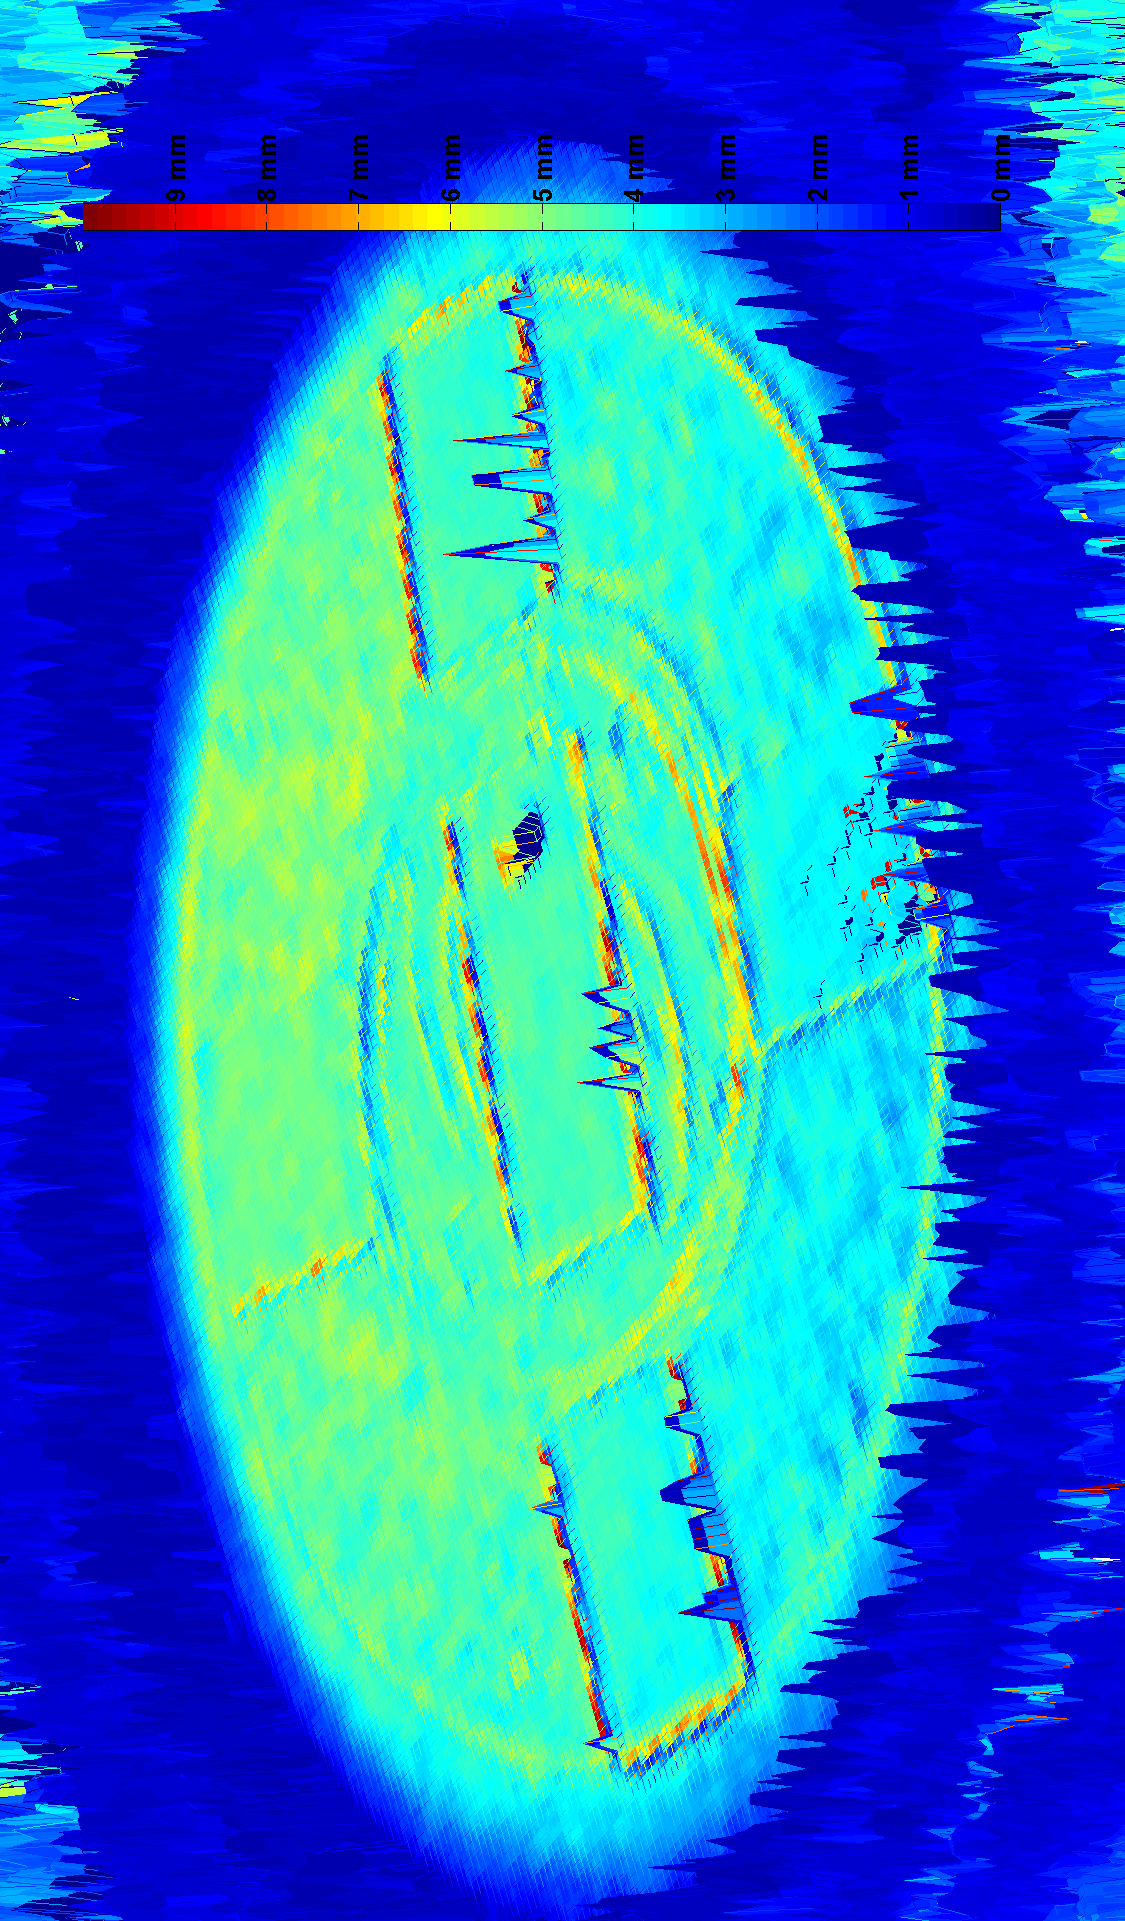
\includegraphics[width=0.6\textwidth]{Bilder/4D_Plot_0_7m.png}
	\caption{Distribution of dominating amplitudes (color) and frequency (z-axis) in $0.7~m$ distance after 8 seconds}
	\label{fig:_Freq_Amp_distribution_3D}
\end{figure}
 
\newpage
\begin{figure}[!h]  
	\centering
	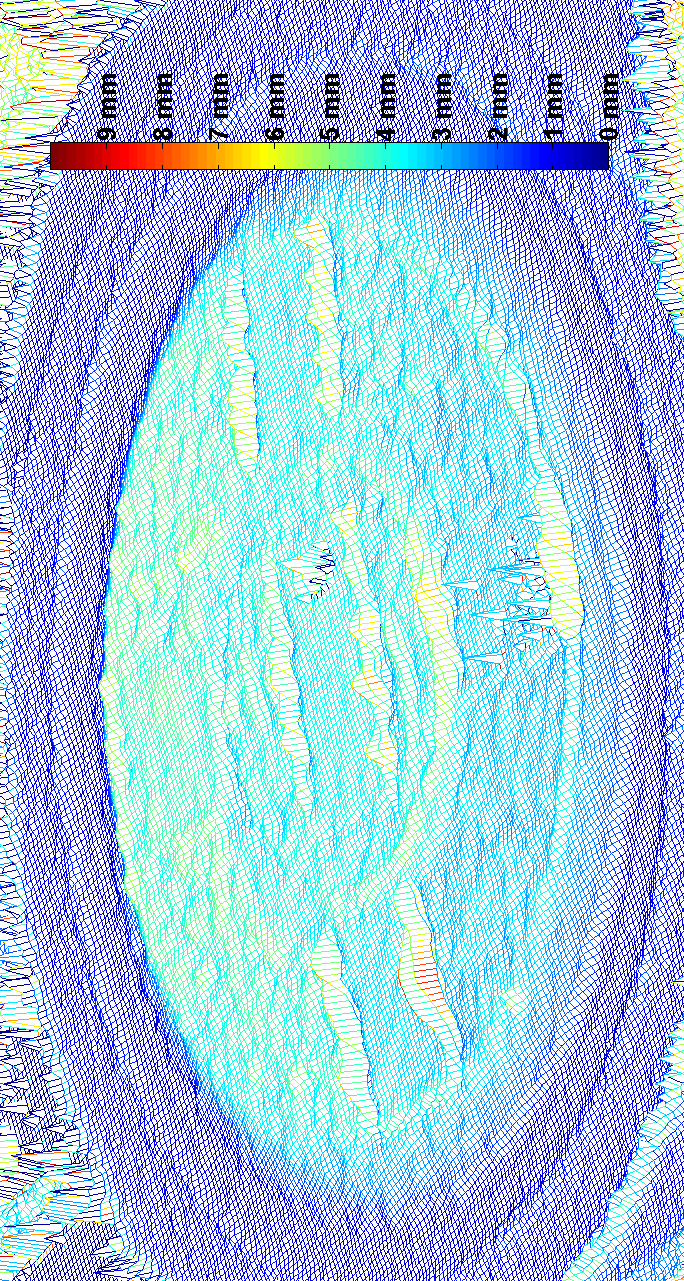
\includegraphics[width=0.70\textwidth]{Bilder/Amp_dis_3D_0_7m.png}
	\caption{Distribution of dominating amplitudes (z-axis) in $0.7~m$  after 8 seconds}
	\label{fig:Amp_distribution_3D}
\end{figure}

\newpage
\begin{table}[!h]
	\begin{center}
		\begin{tabular}{ c  p{8cm}  p{5cm}  }
			\tiny $0^\circ$
			\raisebox{-\totalheight}{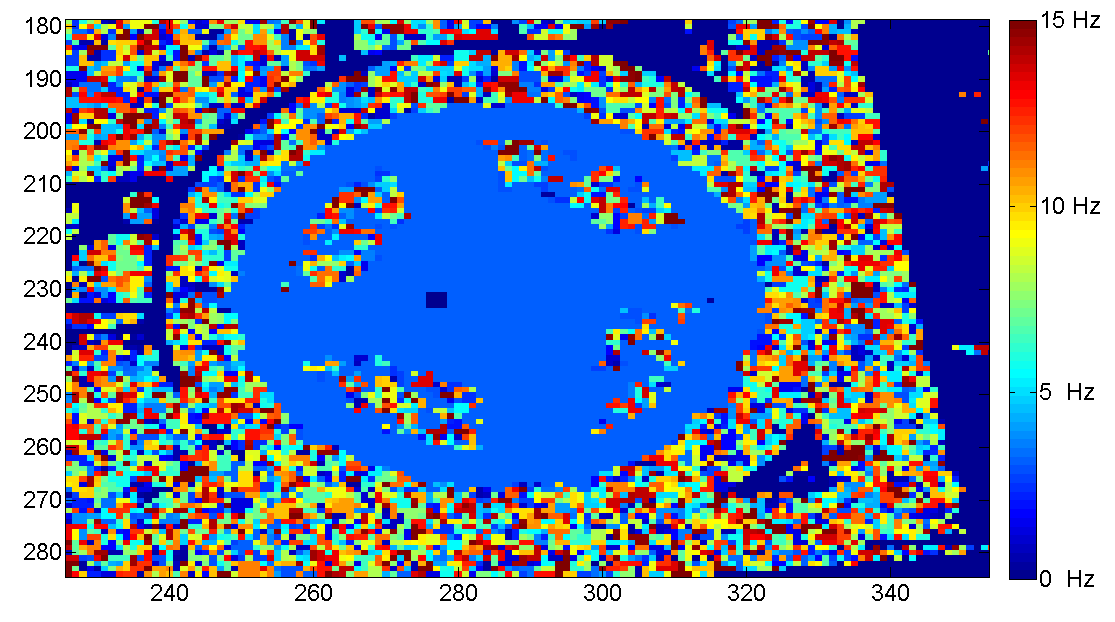
\includegraphics[width=0.5\textwidth]{Bilder/90DEG_freq.png}}
			& 
			\tiny $5^\circ$
			\raisebox{-\totalheight}{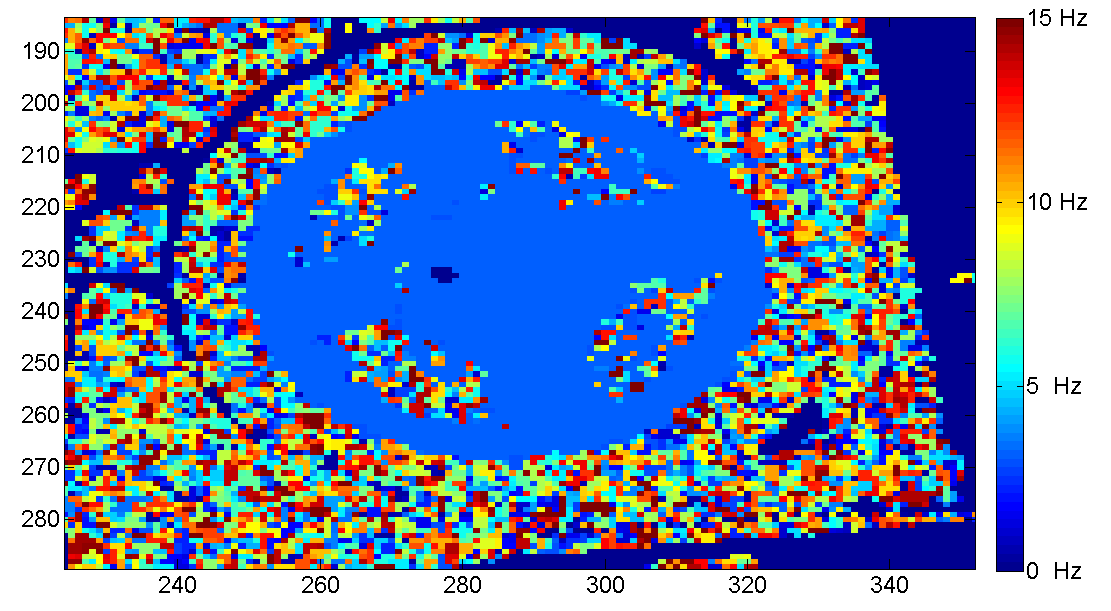
\includegraphics[width=0.5\textwidth]{Bilder/85DEG_freq.png}}\\
			\tiny $10^\circ$
			\raisebox{-\totalheight}{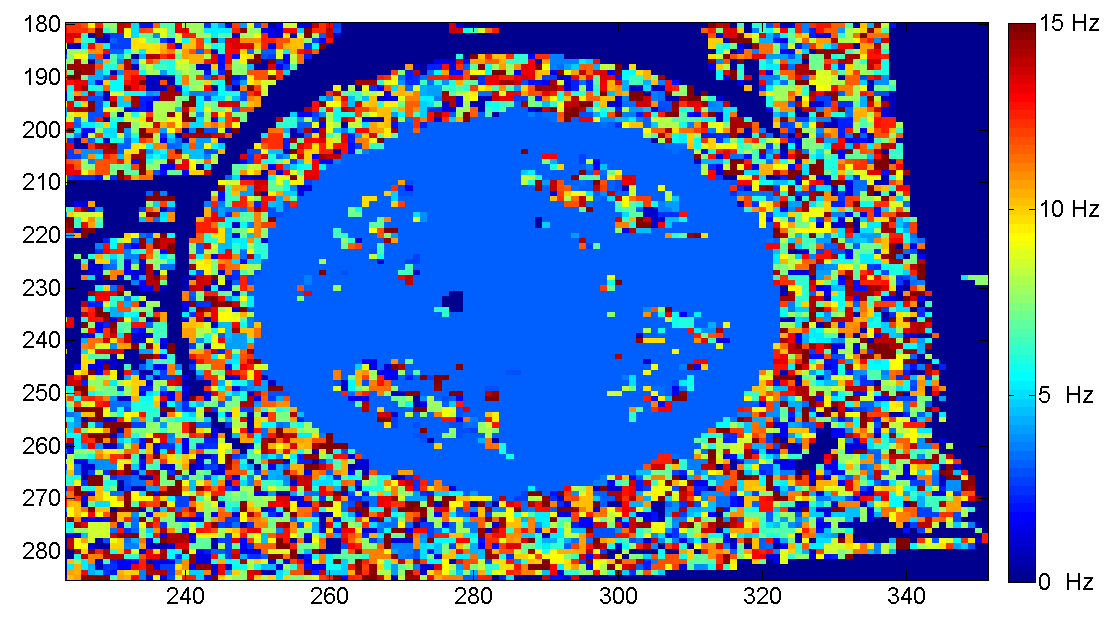
\includegraphics[width=0.5\textwidth]{Bilder/80DEG_freq.png}}
			& 
			\tiny $15^\circ$
			\raisebox{-\totalheight}{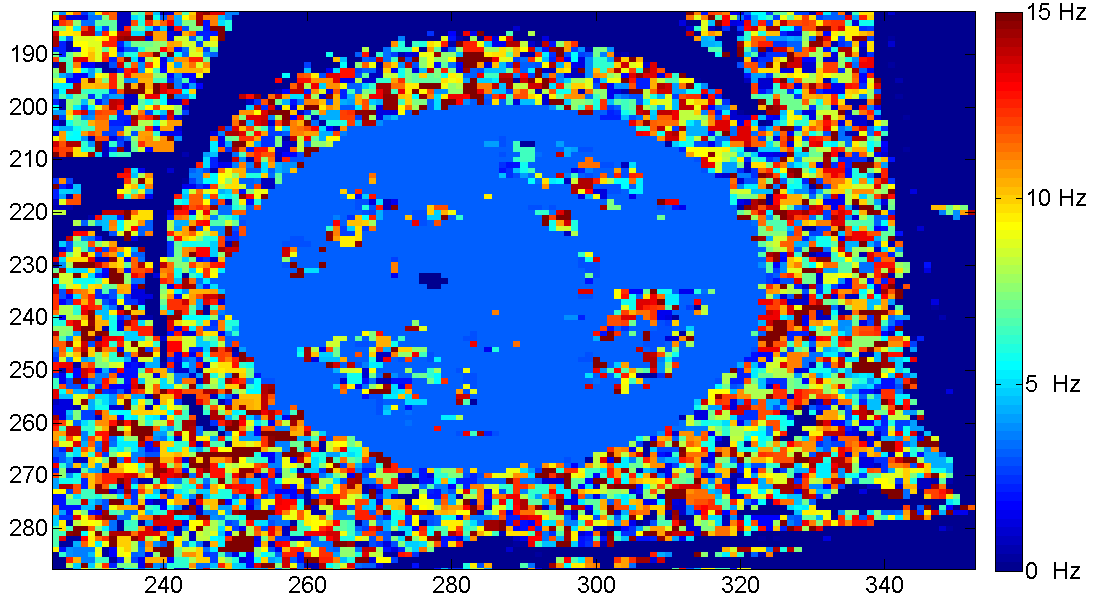
\includegraphics[width=0.5\textwidth]{Bilder/75DEG_freq.png}}\\
			\tiny $20^\circ$
			\raisebox{-\totalheight}{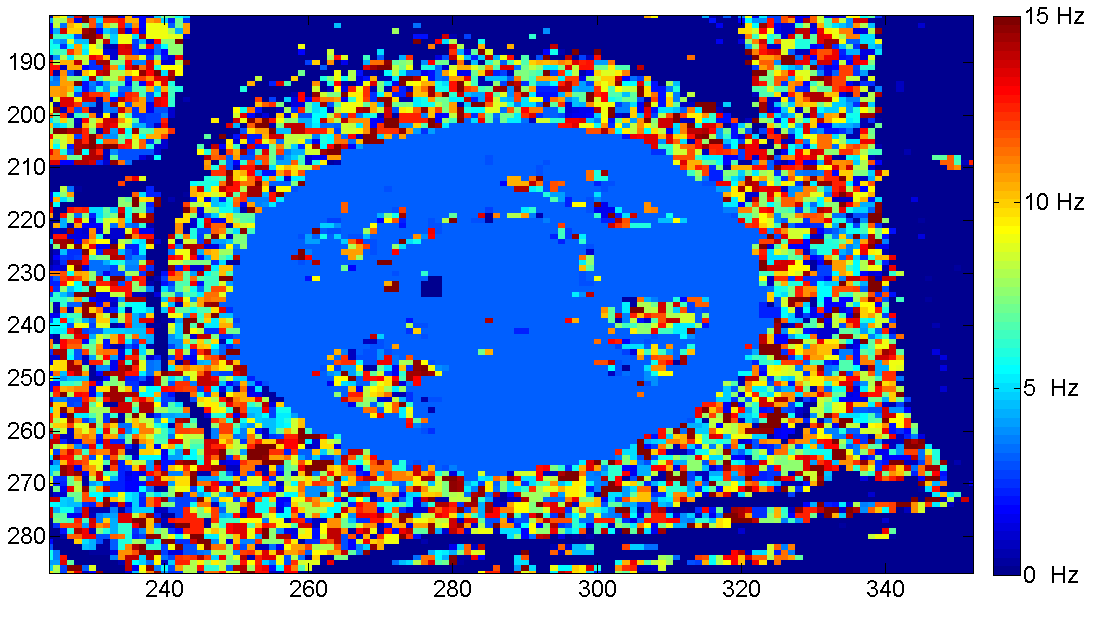
\includegraphics[width=0.5\textwidth]{Bilder/70DEG_freq.png}}
			& 
			\tiny $25^\circ$
			\raisebox{-\totalheight}{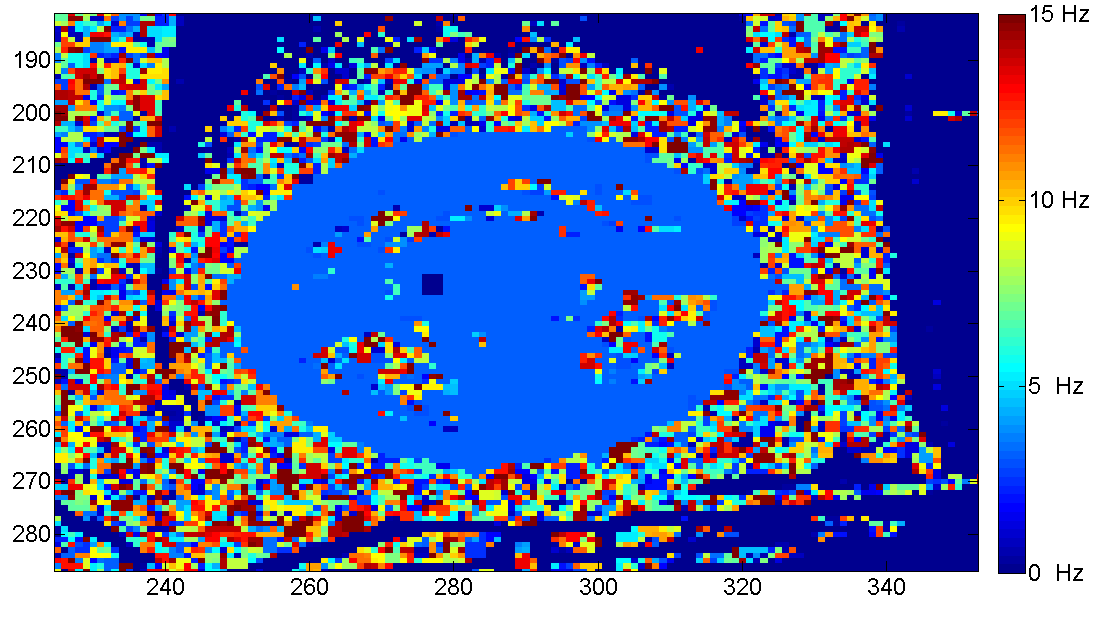
\includegraphics[width=0.5\textwidth]{Bilder/65DEG_freq.png}}\\
			\tiny $30^\circ$
			\raisebox{-\totalheight}{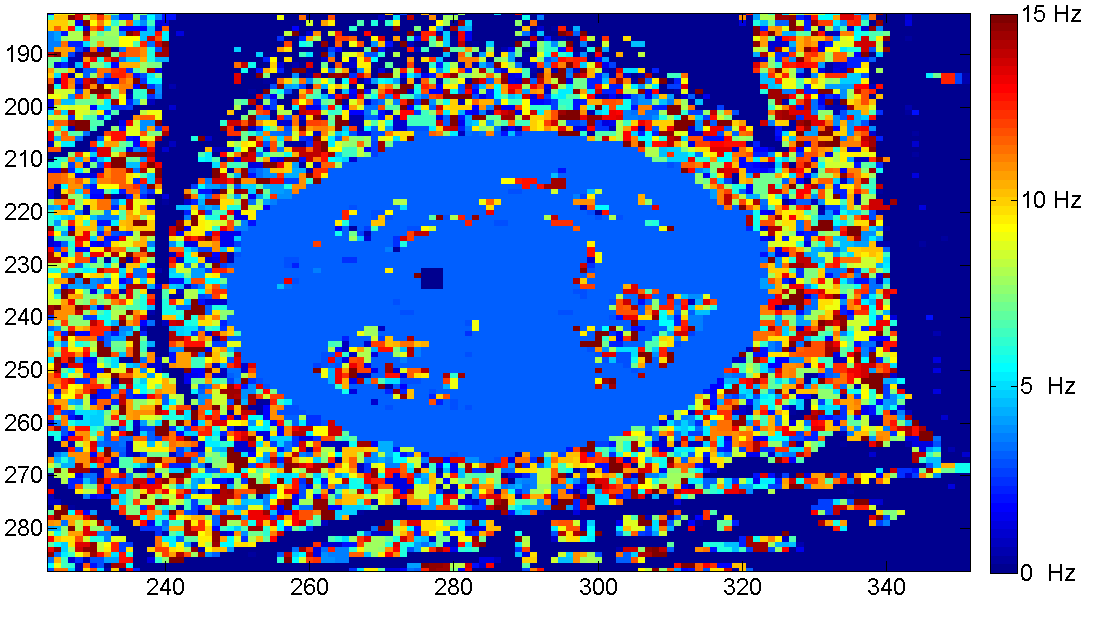
\includegraphics[width=0.5\textwidth]{Bilder/60DEG_freq.png}}
			& 
			\tiny $35^\circ$
			\raisebox{-\totalheight}{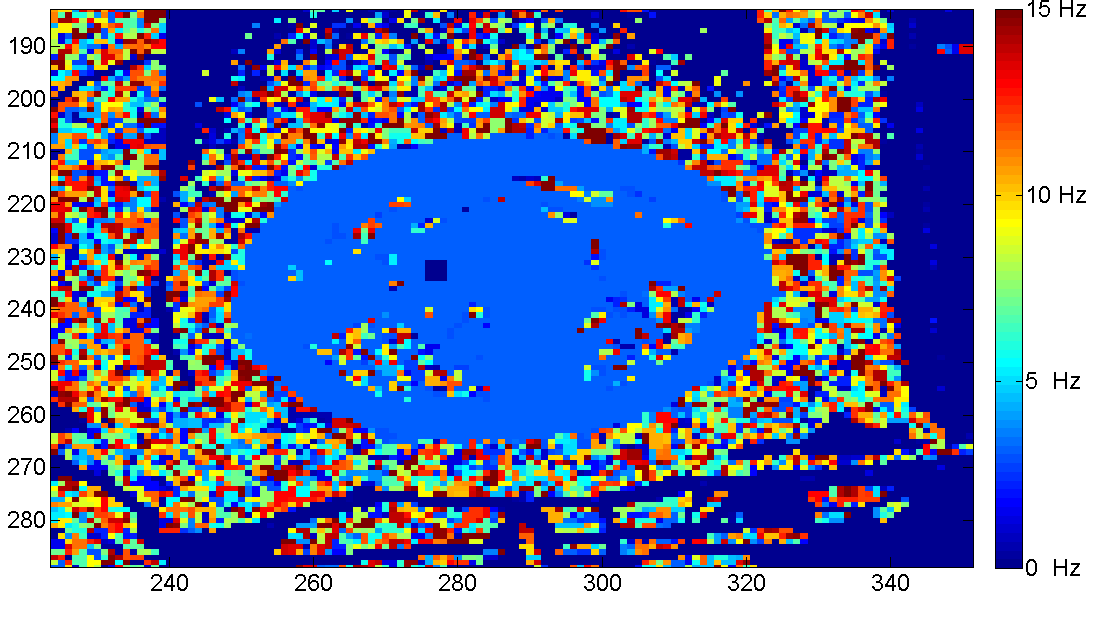
\includegraphics[width=0.5\textwidth]{Bilder/55DEG_freq.png}}
		\end{tabular}
		\caption{Dominating frequency $f_p$ for $0^\circ$ to $35^\circ$ at $1.4~m$ after 8 s}
		\label{tbl:Dominating_freq_angle}
	\end{center}
\end{table}

\newpage
\begin{table}[!h]
	\begin{center}
		\begin{tabular}{ c  p{8cm}  p{5cm}  }
			\tiny $0^\circ$
			\raisebox{-\totalheight}{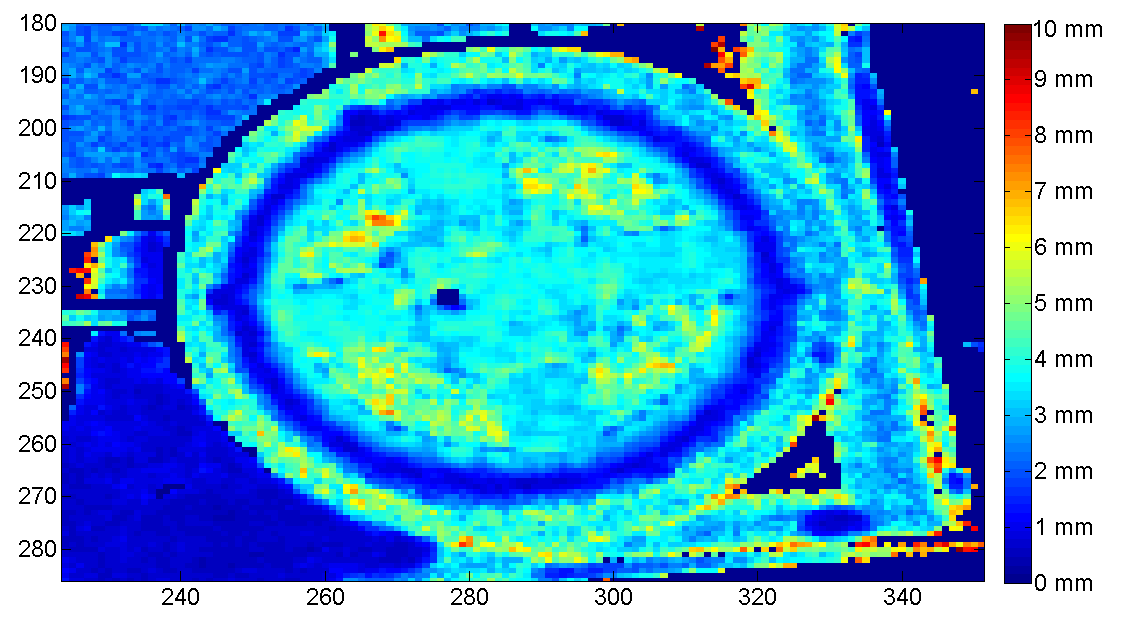
\includegraphics[width=0.5\textwidth]{Bilder/90DEG_Amp.png}}
			& 
			\tiny $5^\circ$
			\raisebox{-\totalheight}{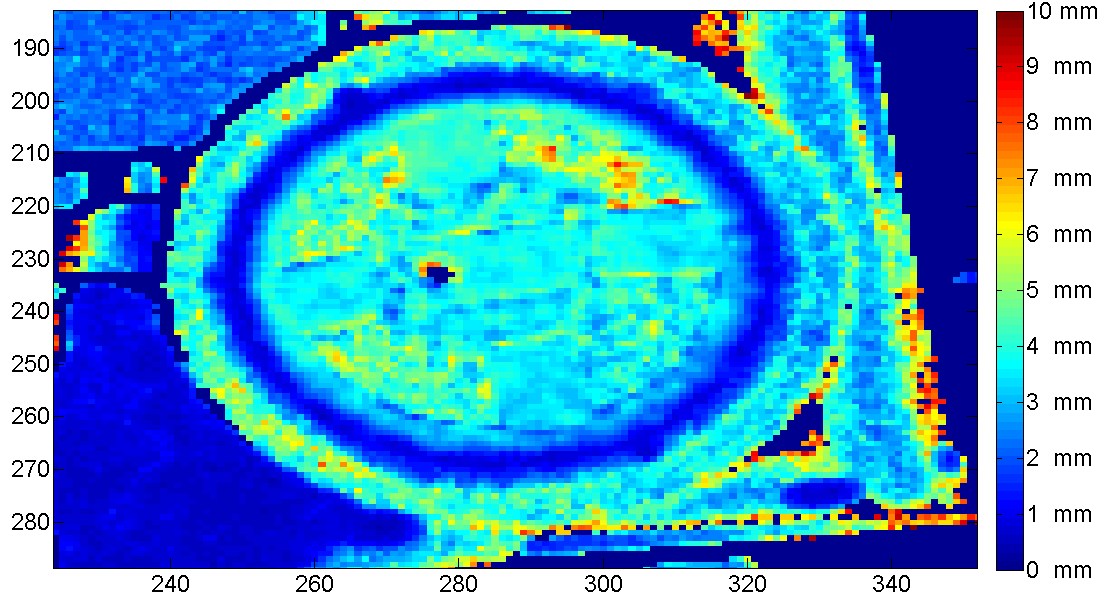
\includegraphics[width=0.5\textwidth]{Bilder/85DEG_Amp.png}}\\
			\tiny $10^\circ$
			\raisebox{-\totalheight}{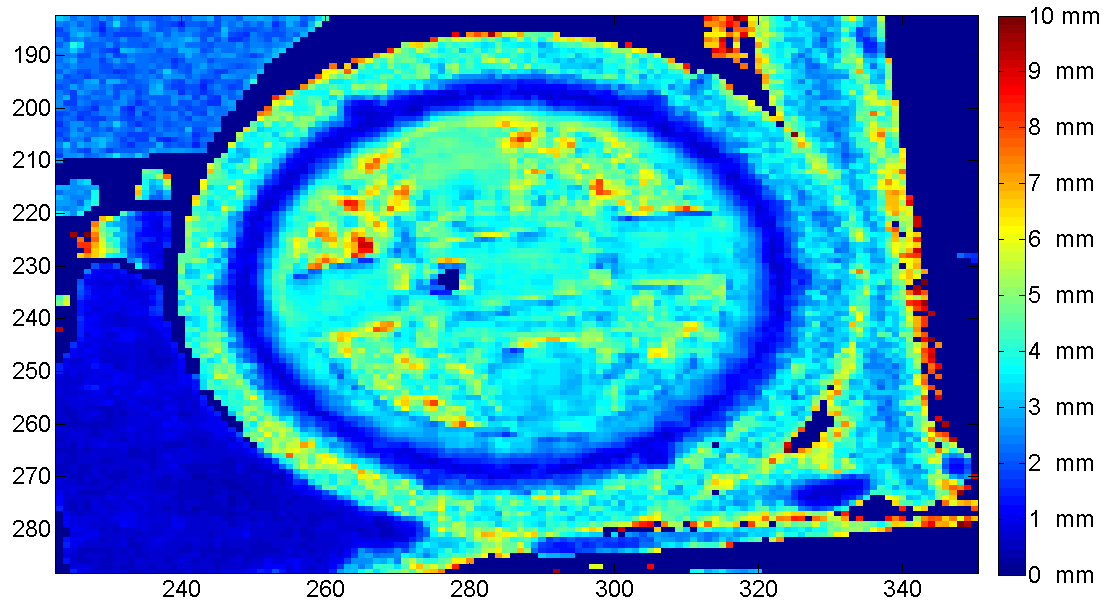
\includegraphics[width=0.5\textwidth]{Bilder/80DEG_Amp.png}}
			& 
			\tiny $15^\circ$
			\raisebox{-\totalheight}{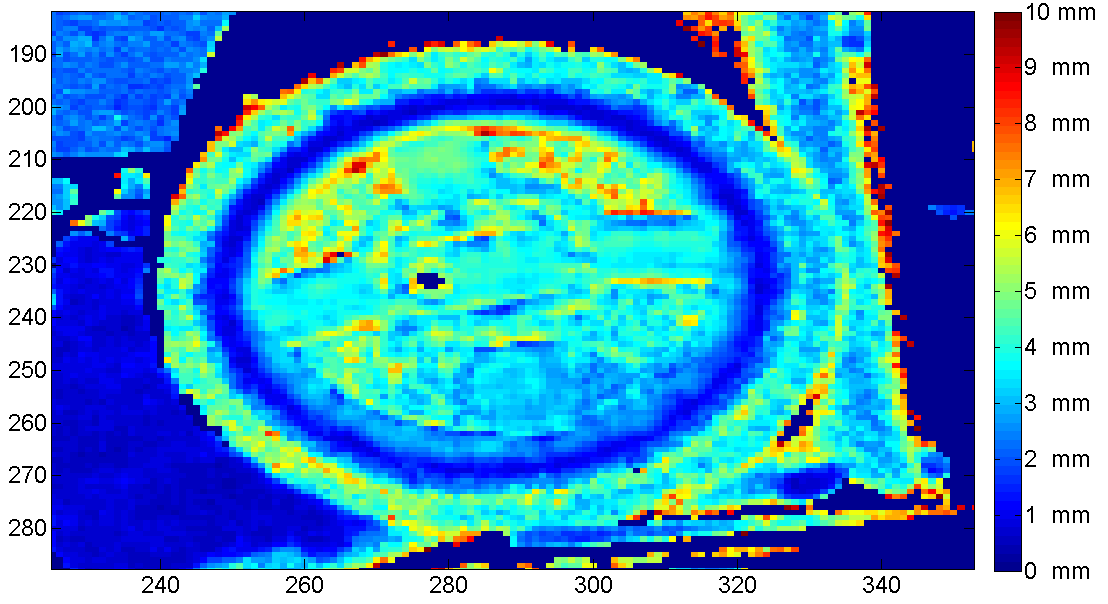
\includegraphics[width=0.5\textwidth]{Bilder/75DEG_Amp.png}}\\
			\tiny $20^\circ$
			\raisebox{-\totalheight}{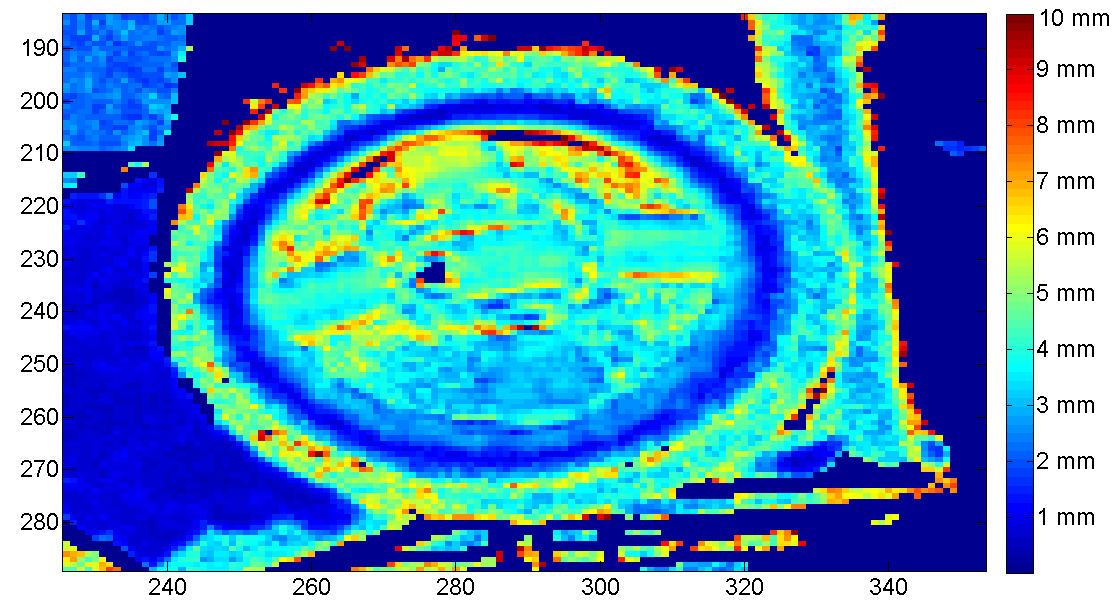
\includegraphics[width=0.5\textwidth]{Bilder/70DEG_Amp.png}}
			& 
			\tiny $25^\circ$
			\raisebox{-\totalheight}{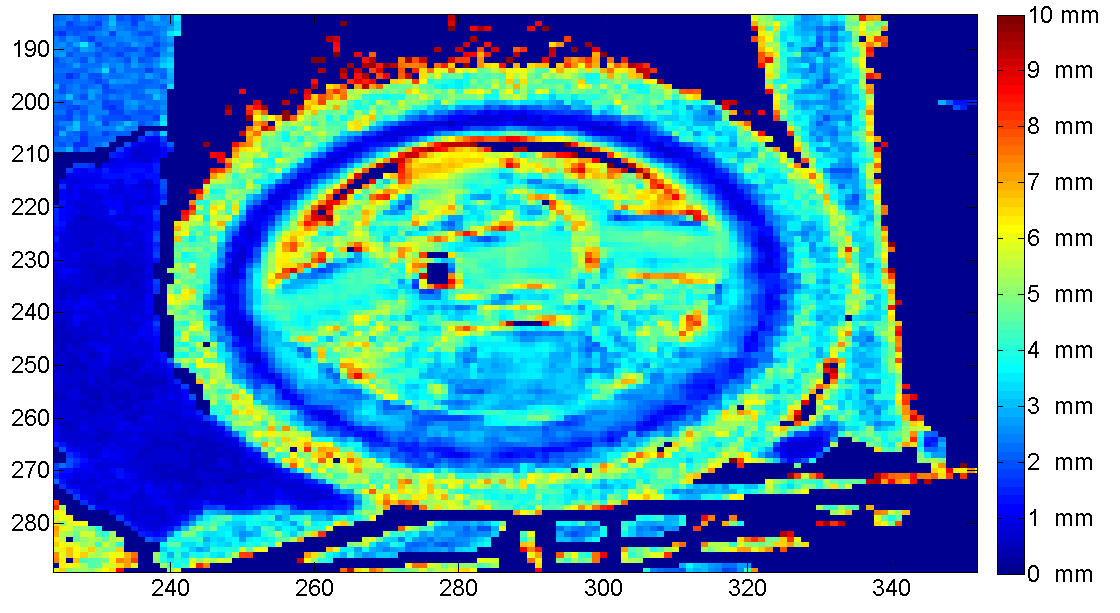
\includegraphics[width=0.5\textwidth]{Bilder/65DEG_Amp.png}}\\
			\tiny $30^\circ$
			\raisebox{-\totalheight}{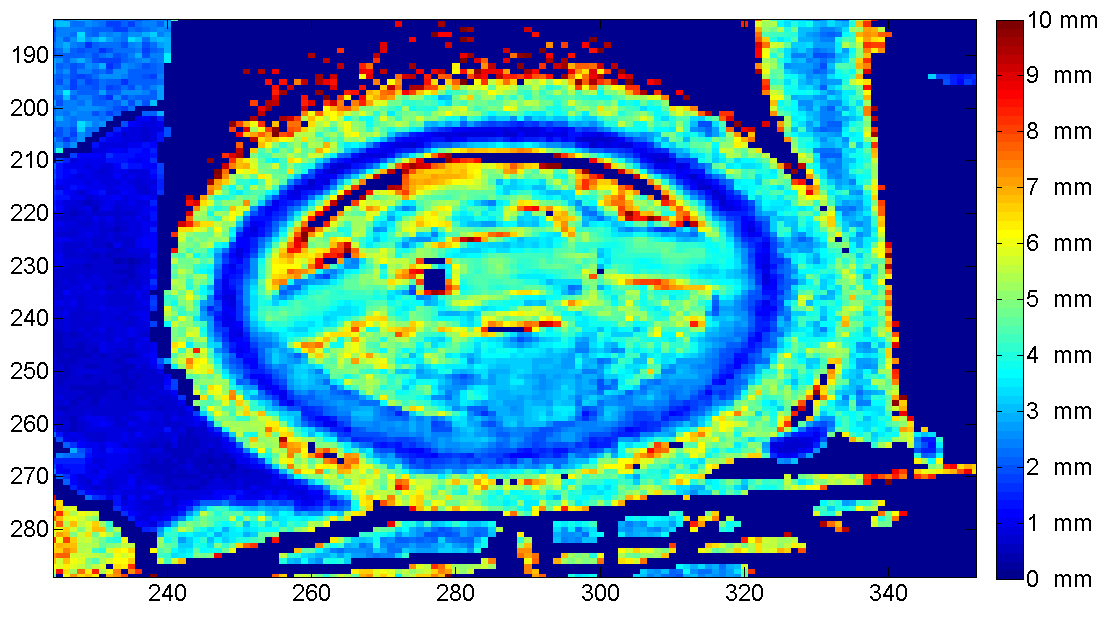
\includegraphics[width=0.5\textwidth]{Bilder/60DEG_Amp.png}}
			&
			\tiny $35^\circ$ 
			\raisebox{-\totalheight}{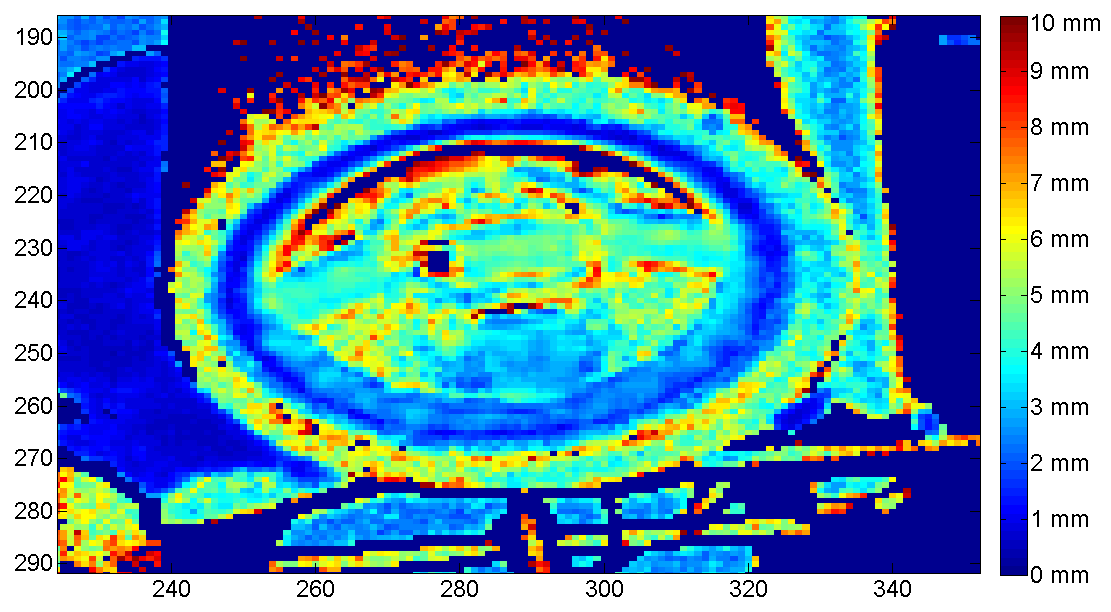
\includegraphics[width=0.5\textwidth]{Bilder/55DEG_Amp.png}}
		\end{tabular}
		\caption{Dominating amplitude $A_p$ for $0^\circ$ to $35^\circ$ at $1.4~m$ after 8 s}
		\label{tbl:Dominating_amp_angle}
	\end{center}
\end{table}
\newpage
\begin{table}[!h]
	\begin{center}
		\begin{tabular}{ c  p{8cm}  p{5cm}  }
			\tiny $0.6~m$
			\raisebox{-\totalheight}{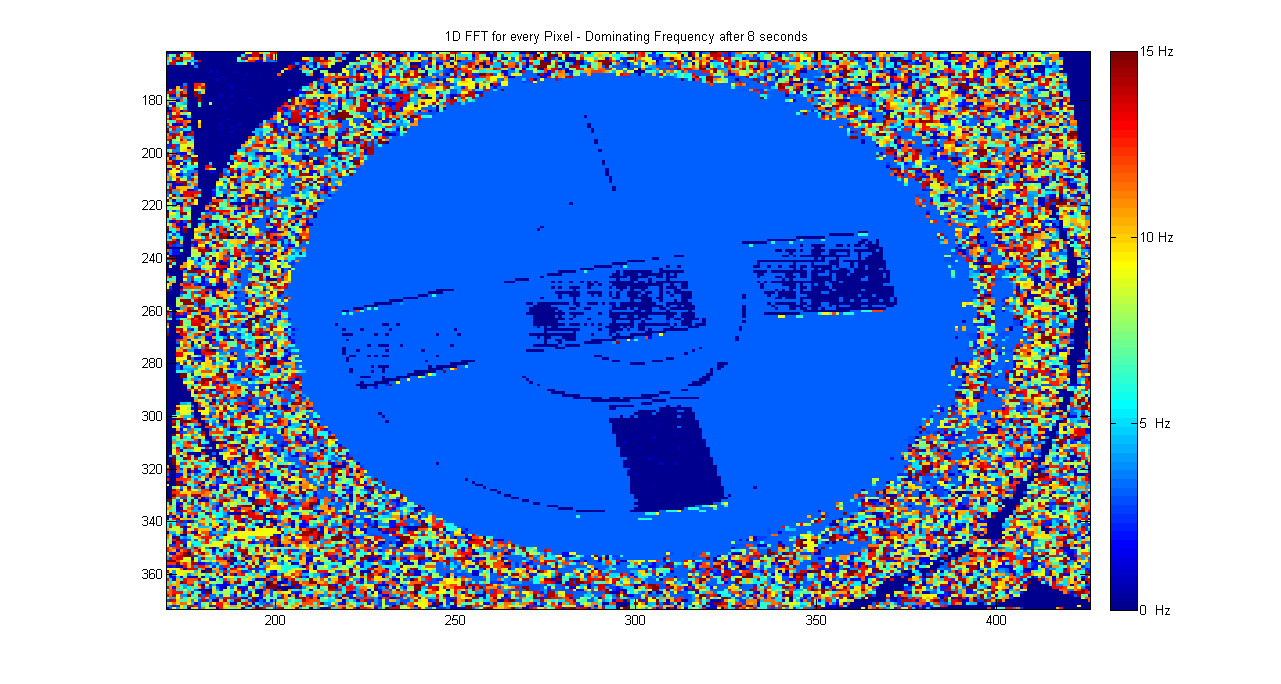
\includegraphics[width=0.5\textwidth]{Bilder/0_6m_Freq.png}}
			&
			\tiny $0.7~m$ 
			\raisebox{-\totalheight}{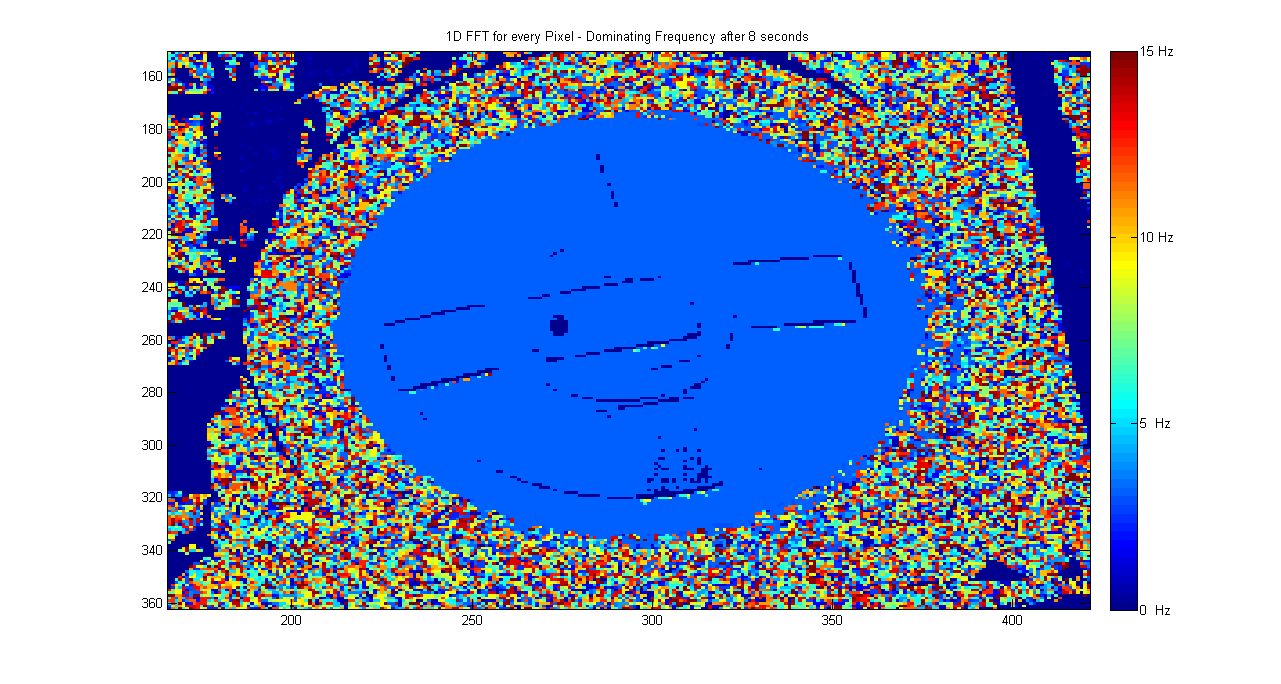
\includegraphics[width=0.5\textwidth]{Bilder/0_7m_Freq.png}}\\
			\tiny $0.8~m$
			\raisebox{-\totalheight}{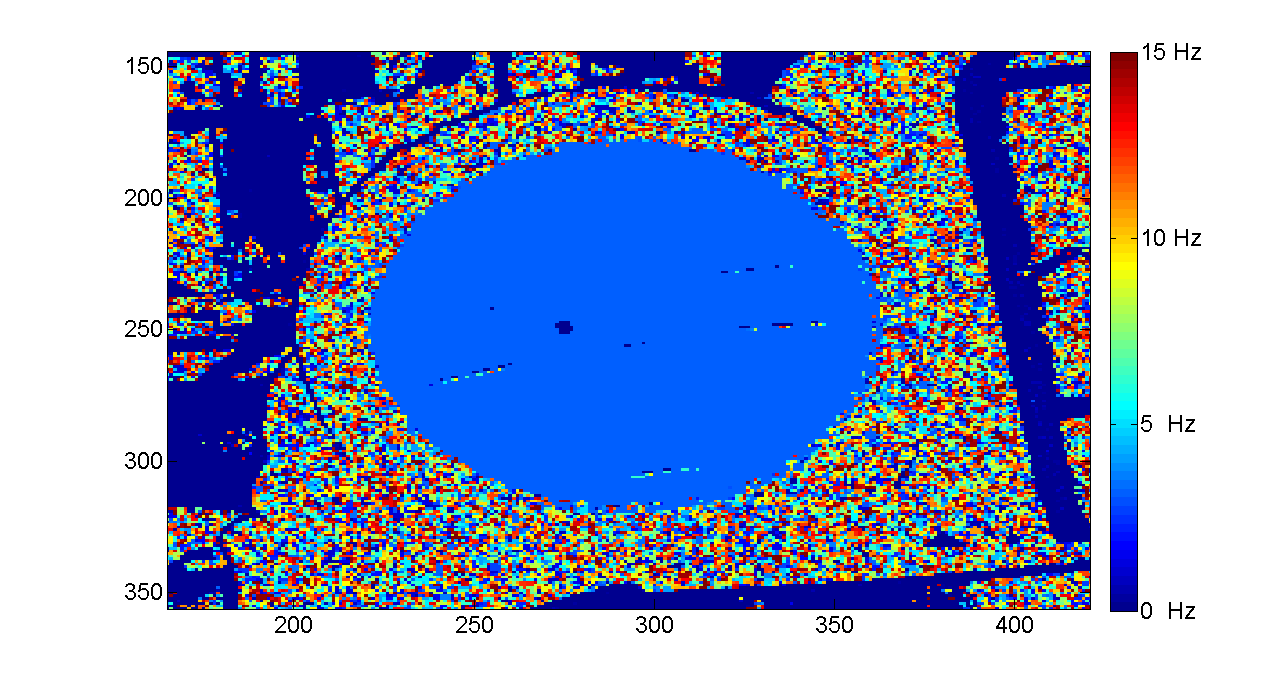
\includegraphics[width=0.5\textwidth]{Bilder/0_8m_Freq.png}}
			& 
			\tiny $0.9~m$
			\raisebox{-\totalheight}{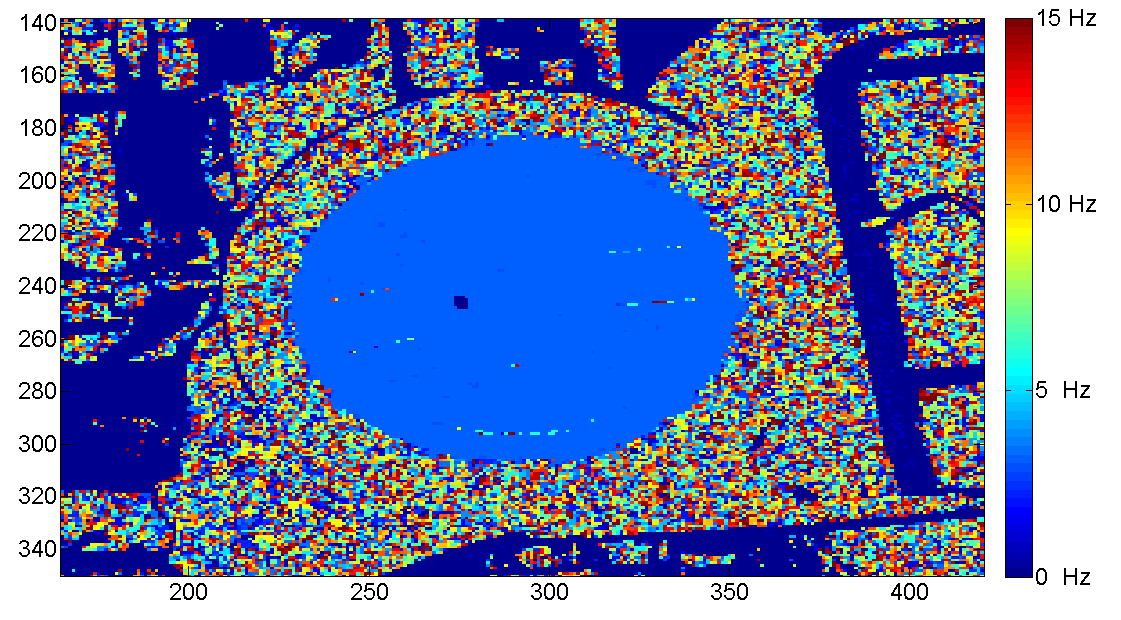
\includegraphics[width=0.5\textwidth]{Bilder/0_9m_Freq.png}}\\
			\tiny $1.0~m$
			\raisebox{-\totalheight}{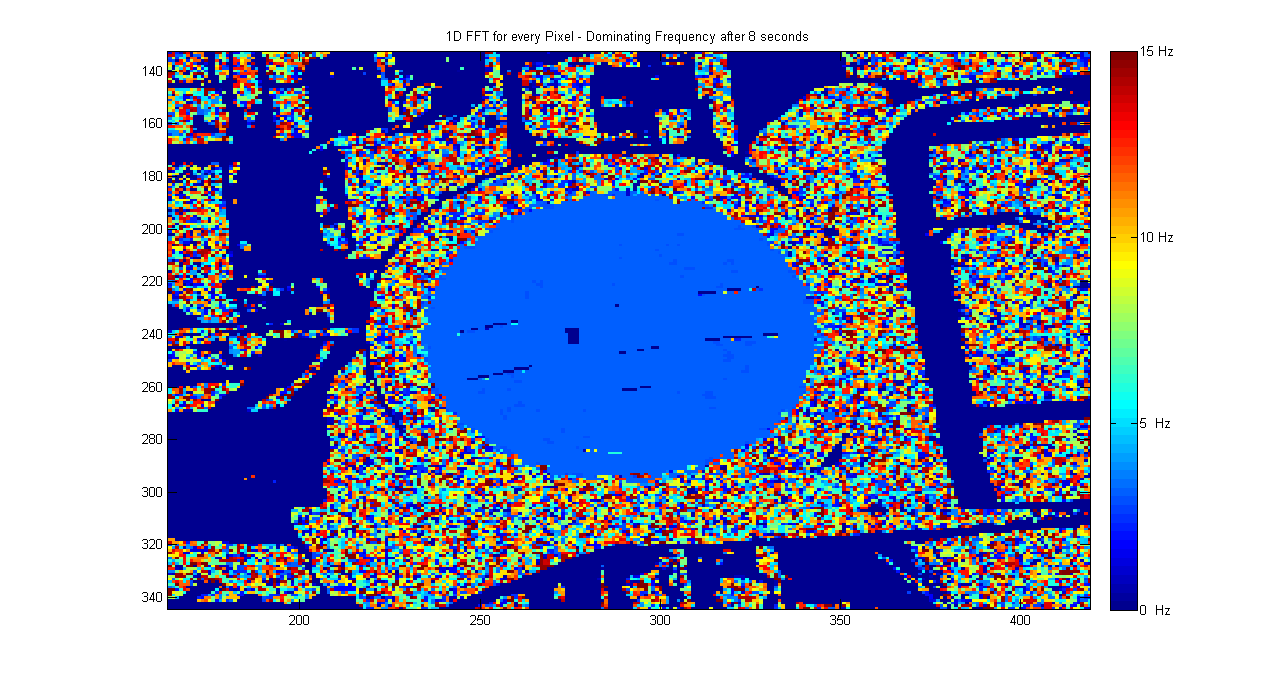
\includegraphics[width=0.5\textwidth]{Bilder/1_0m_Freq.png}}
			& 
			\tiny $1.1~m$
			\raisebox{-\totalheight}{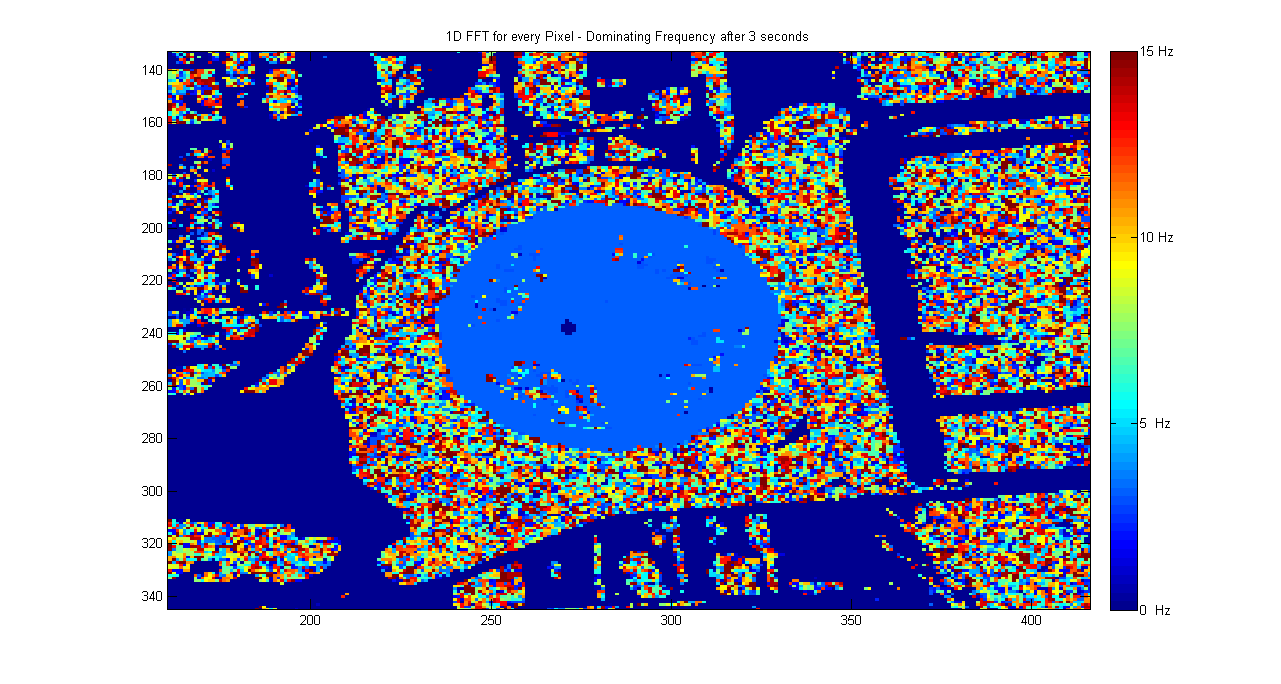
\includegraphics[width=0.5\textwidth]{Bilder/1_1m_Freq.png}}\\
			\tiny $1.2~m$
			\raisebox{-\totalheight}{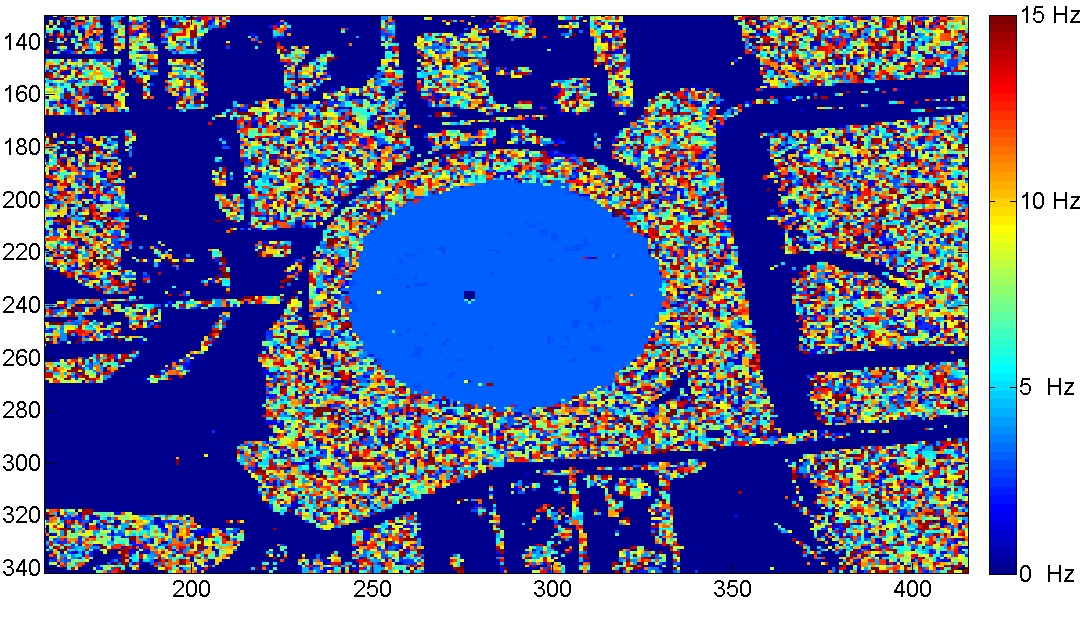
\includegraphics[width=0.5\textwidth]{Bilder/1_2m_Freq.png}}
			& 
			\tiny $1.3~m$
			\raisebox{-\totalheight}{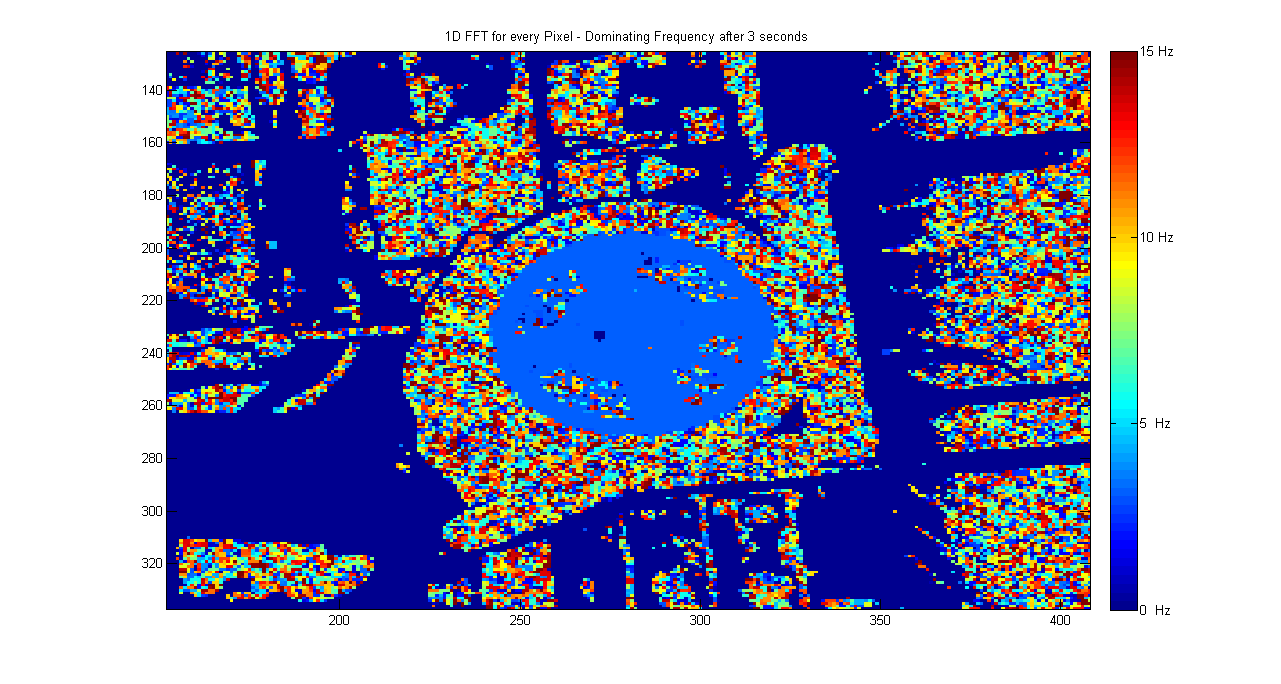
\includegraphics[width=0.5\textwidth]{Bilder/1_3m_Freq.png}}
		\end{tabular}
		\caption{Dominating frequency $f_p$ in a distance of $0.6~m$ to $1.3~m$ after 8 s}
		\label{tbl:Dominating_freq_distance}
	\end{center}
\end{table}

\newpage
\begin{table}[!h]
	\begin{center}
		\begin{tabular}{ c  p{8cm}  p{5cm}  }
			\tiny $0.6~m$
			\raisebox{-\totalheight}{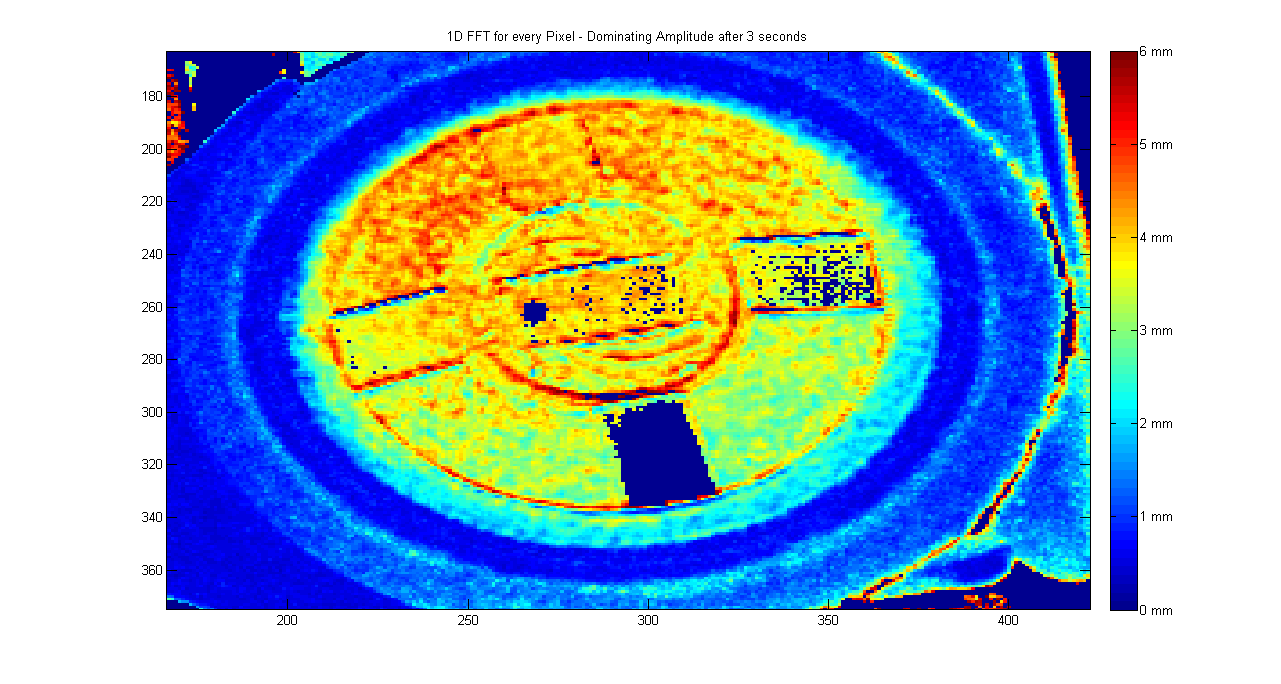
\includegraphics[width=0.5\textwidth]{Bilder/0_6m_Amp.png}}
			&
			\tiny $0.7~m$  
			\raisebox{-\totalheight}{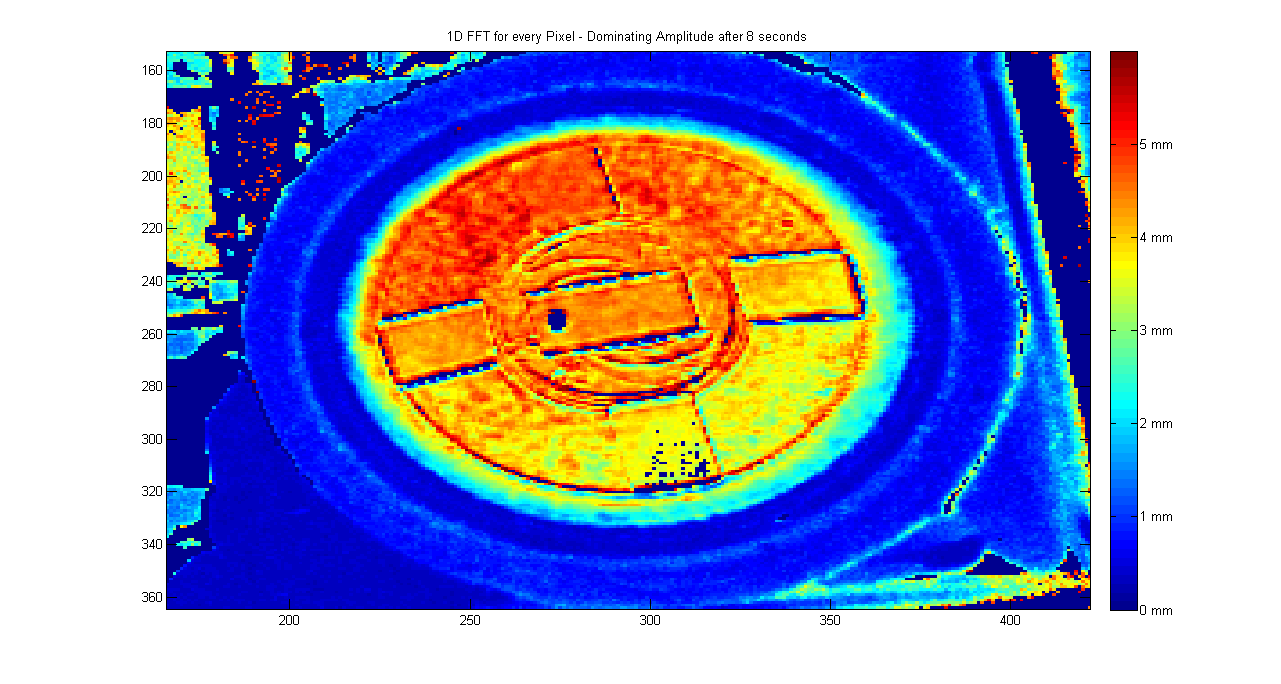
\includegraphics[width=0.5\textwidth]{Bilder/0_7m_Amp.png}}\\
			\tiny $0.8~m$
			\raisebox{-\totalheight}{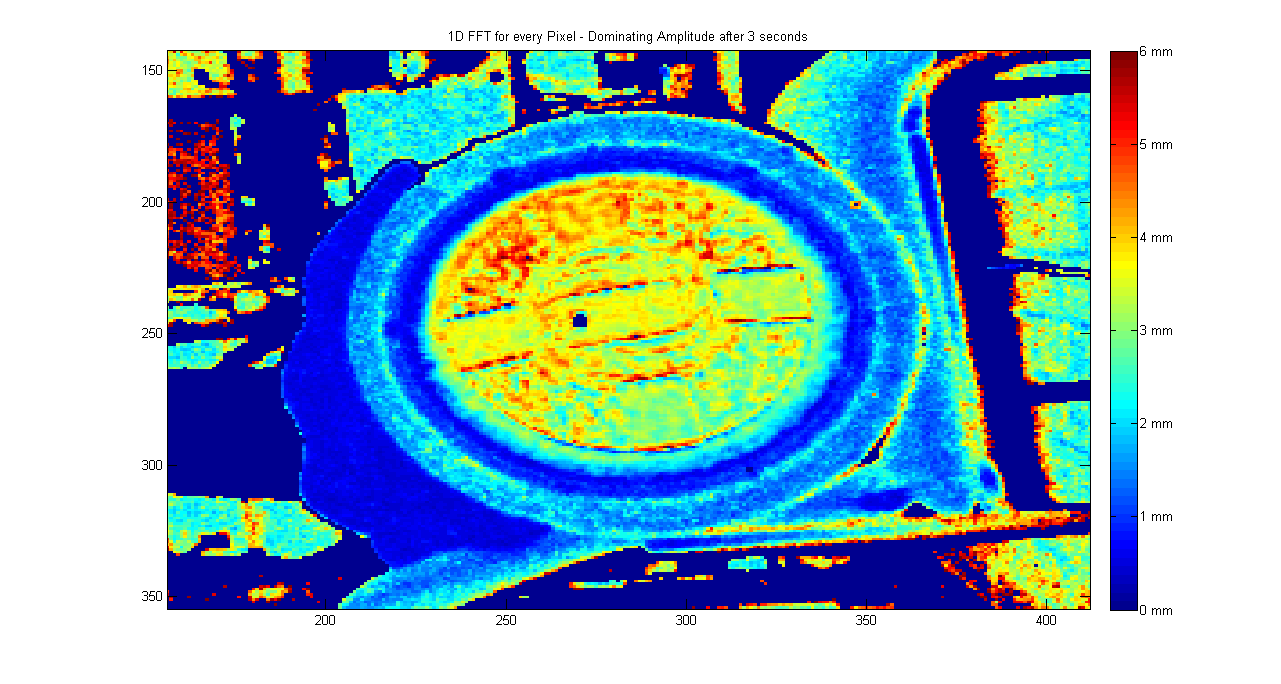
\includegraphics[width=0.5\textwidth]{Bilder/0_8m_Amp.png}}
			& 
			\tiny $0.9~m$
			\raisebox{-\totalheight}{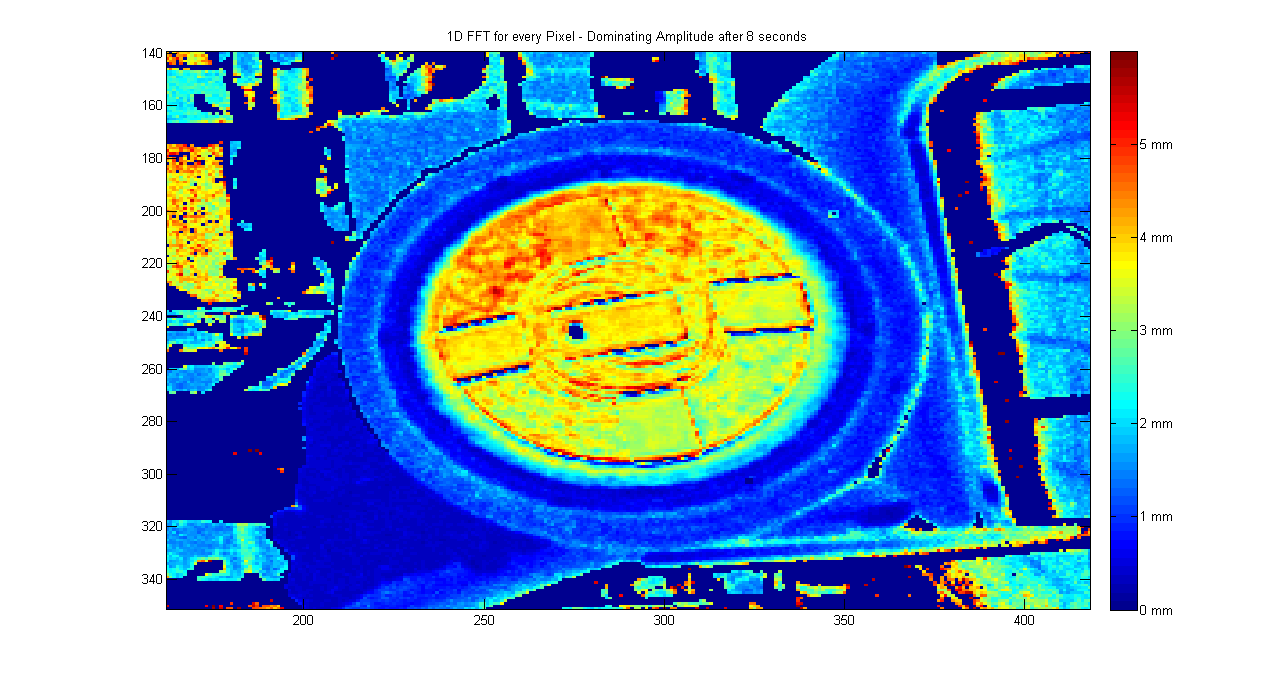
\includegraphics[width=0.5\textwidth]{Bilder/0_9m_Amp.png}}\\
			\tiny $1.0~m$
			\raisebox{-\totalheight}{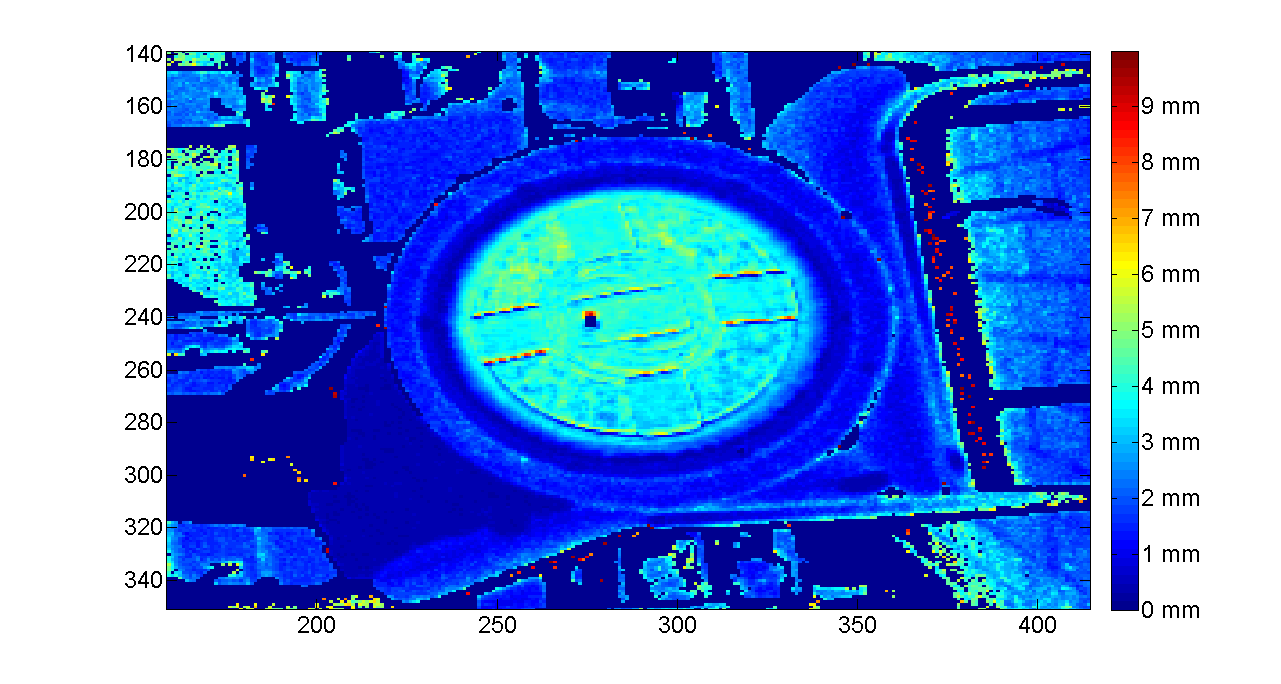
\includegraphics[width=0.5\textwidth]{Bilder/1_0m_Amp.png}}
			& 
			\tiny $1.1~m$
			\raisebox{-\totalheight}{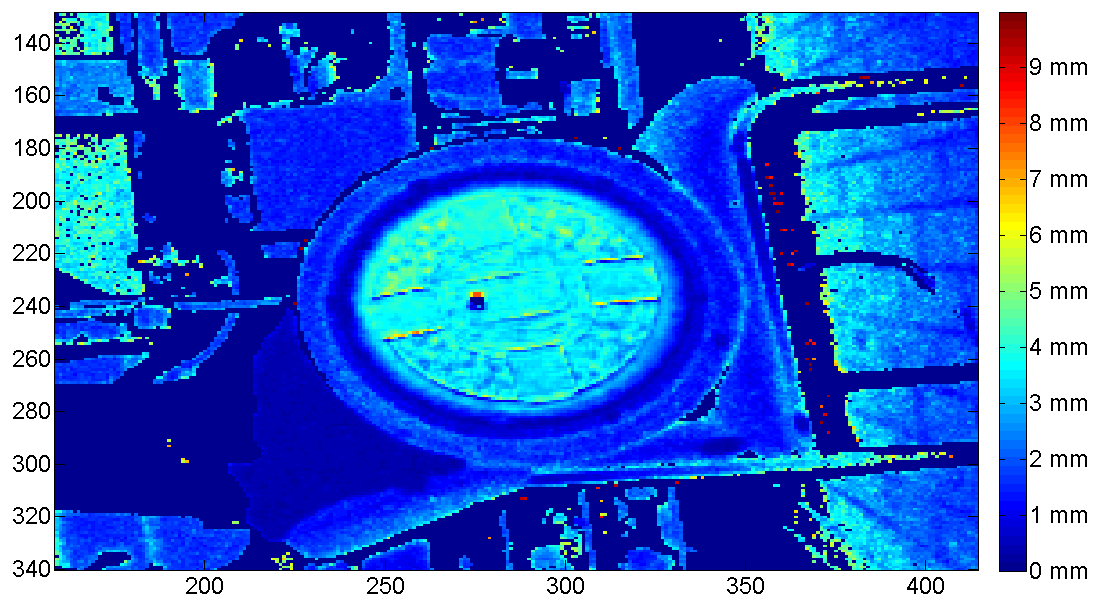
\includegraphics[width=0.5\textwidth]{Bilder/1_1m_Amp.png}}\\
			\tiny $1.2~m$
			\raisebox{-\totalheight}{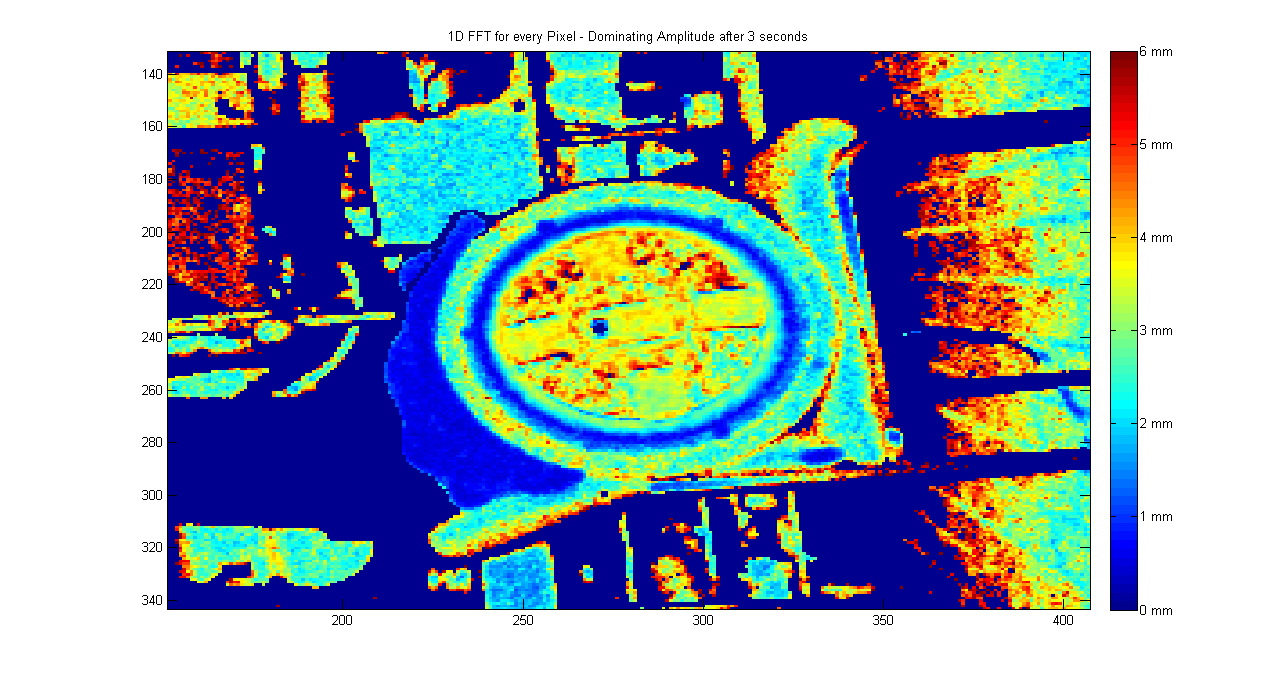
\includegraphics[width=0.5\textwidth]{Bilder/1_2m_Amp.png}}
			&
			\tiny $1.3~m$ 
			\raisebox{-\totalheight}{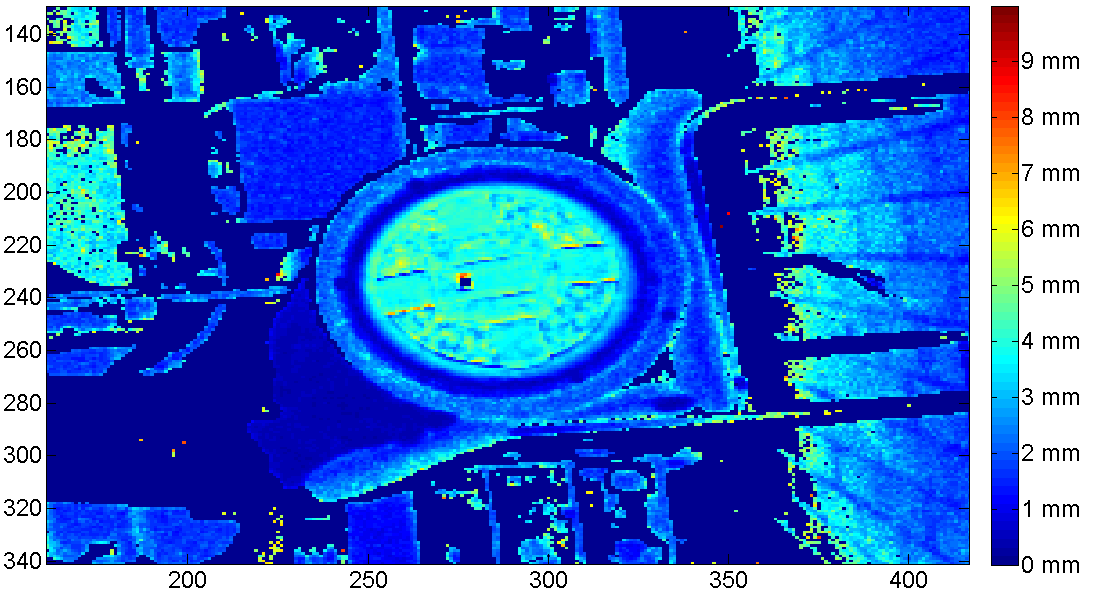
\includegraphics[width=0.5\textwidth]{Bilder/1_3m_Amp.png}}
		\end{tabular}
		\caption{Dominating amplitude $A_p$ in a distance of $0.6~m$ to $1.3~m$ after 8 s}
		\label{tbl:Dominating_amp_distance}
	\end{center}
\end{table}

\newpage
\begin{table}[!h]
	\begin{center}
		\begin{tabular}{ c  p{8cm}  p{5cm}  }
			\tiny $2~Hz$
			\raisebox{-\totalheight}{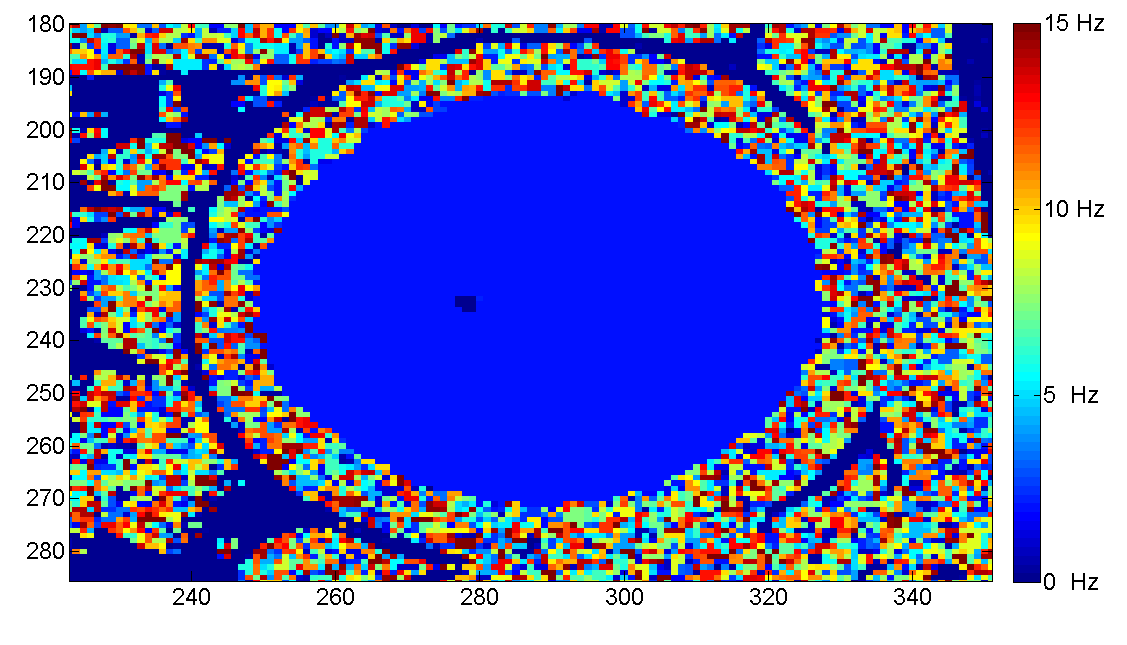
\includegraphics[width=0.5\textwidth]{Bilder/2_Hz_freq.png}}
			&
			\tiny $4~Hz$ 
			\raisebox{-\totalheight}{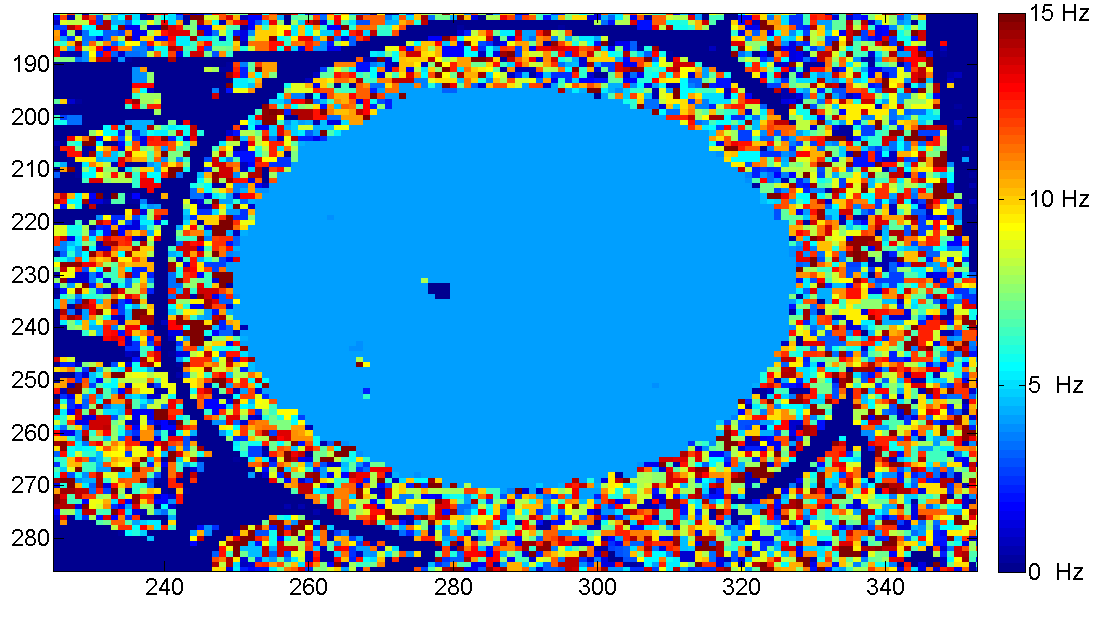
\includegraphics[width=0.5\textwidth]{Bilder/4_Hz_freq.png}}\\
			\tiny $5~Hz$
			\raisebox{-\totalheight}{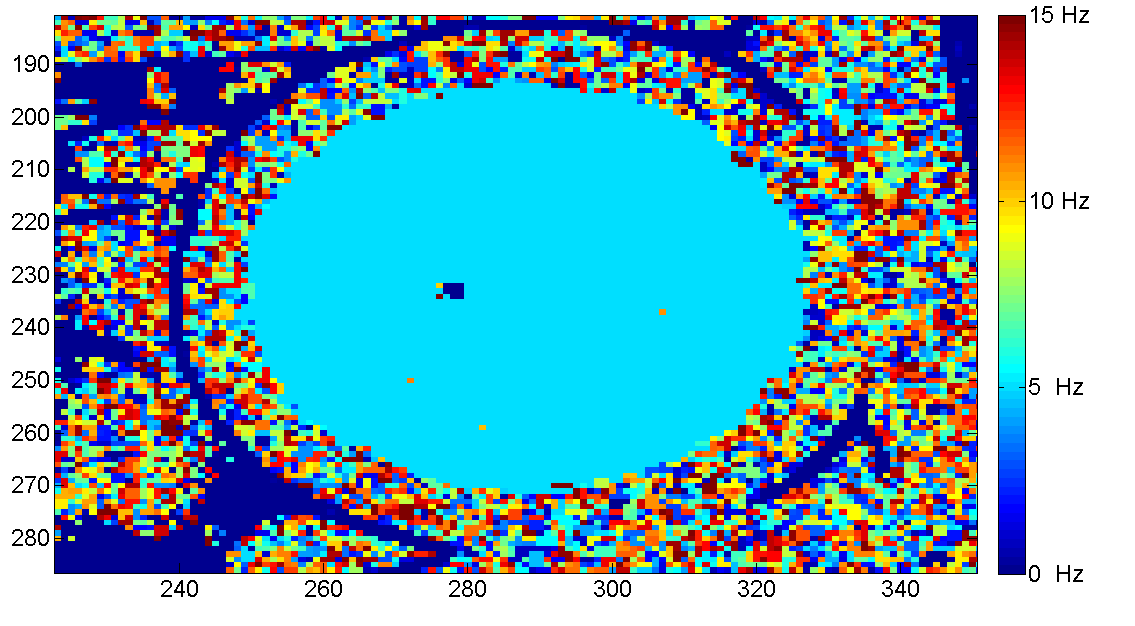
\includegraphics[width=0.5\textwidth]{Bilder/5_Hz_freq.png}}
			& 
			\tiny $6~Hz$
			\raisebox{-\totalheight}{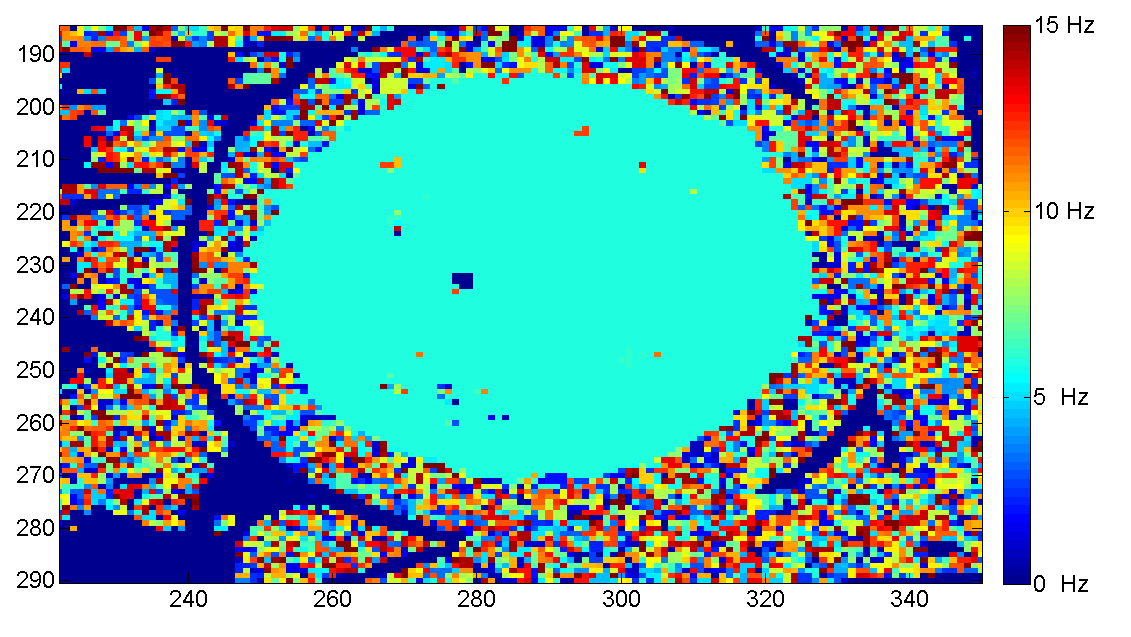
\includegraphics[width=0.5\textwidth]{Bilder/6_Hz_freq.png}}\\
			\tiny $7~Hz$
			\raisebox{-\totalheight}{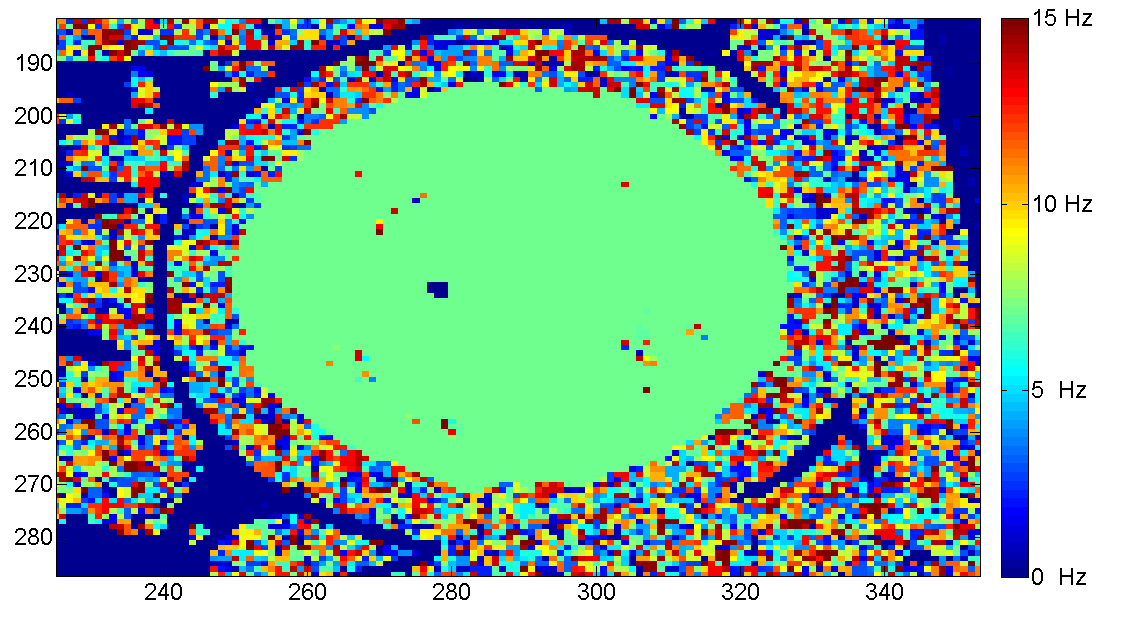
\includegraphics[width=0.5\textwidth]{Bilder/7_Hz_freq.png}}
			& 
			\tiny $8~Hz$
			\raisebox{-\totalheight}{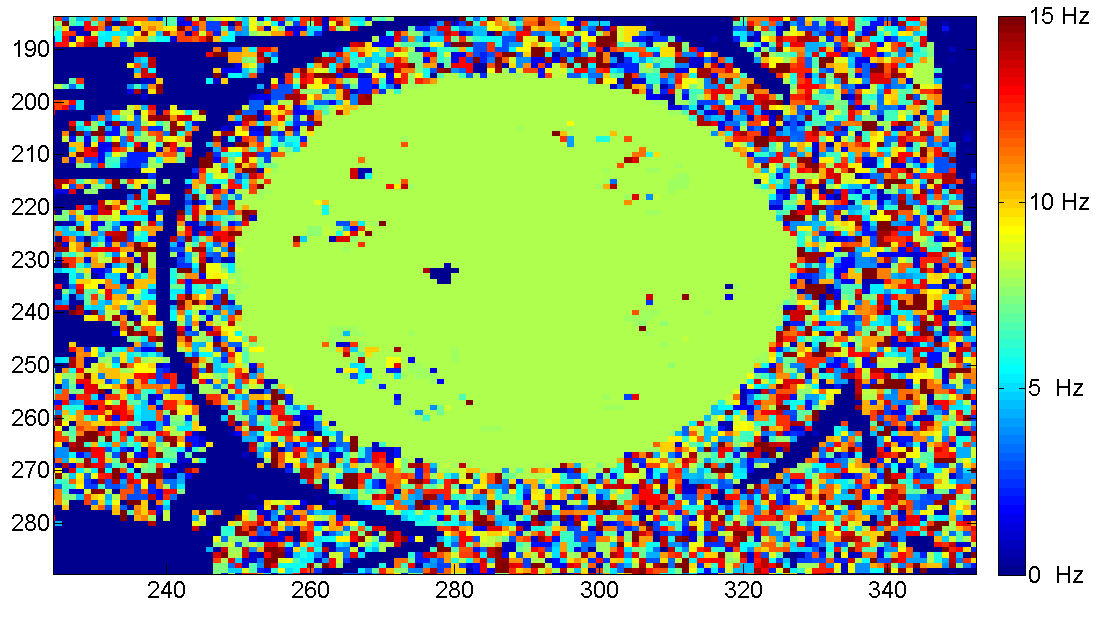
\includegraphics[width=0.5\textwidth]{Bilder/8_Hz_freq.png}}\\
			\tiny $9~Hz$
			\raisebox{-\totalheight}{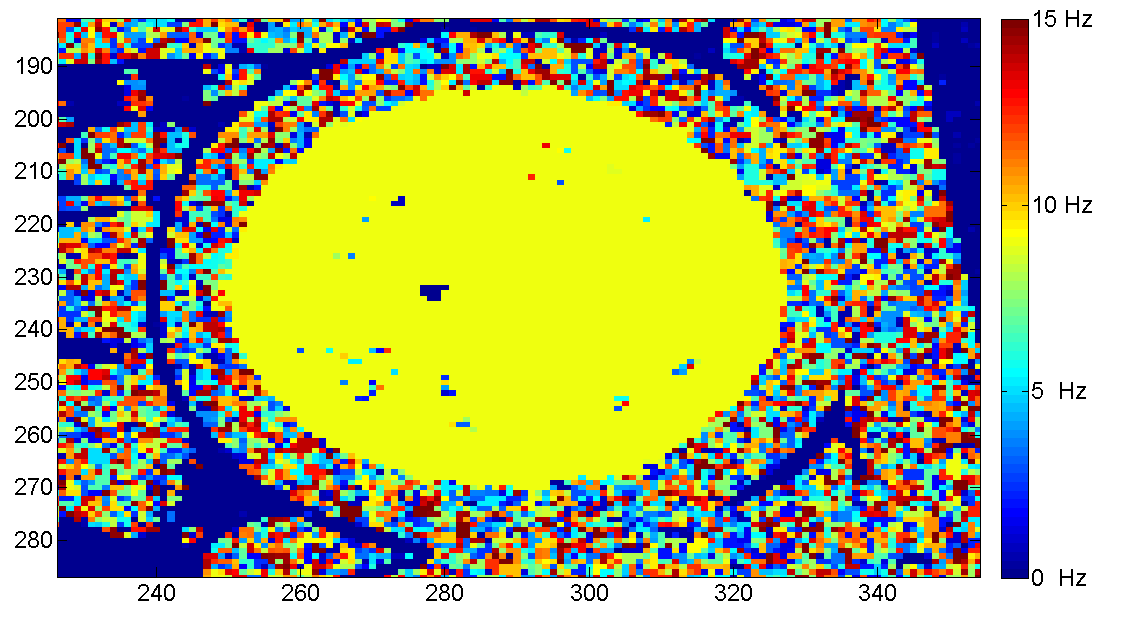
\includegraphics[width=0.5\textwidth]{Bilder/9_Hz_freq.png}}
			&
			\tiny $10~Hz$ 
			\raisebox{-\totalheight}{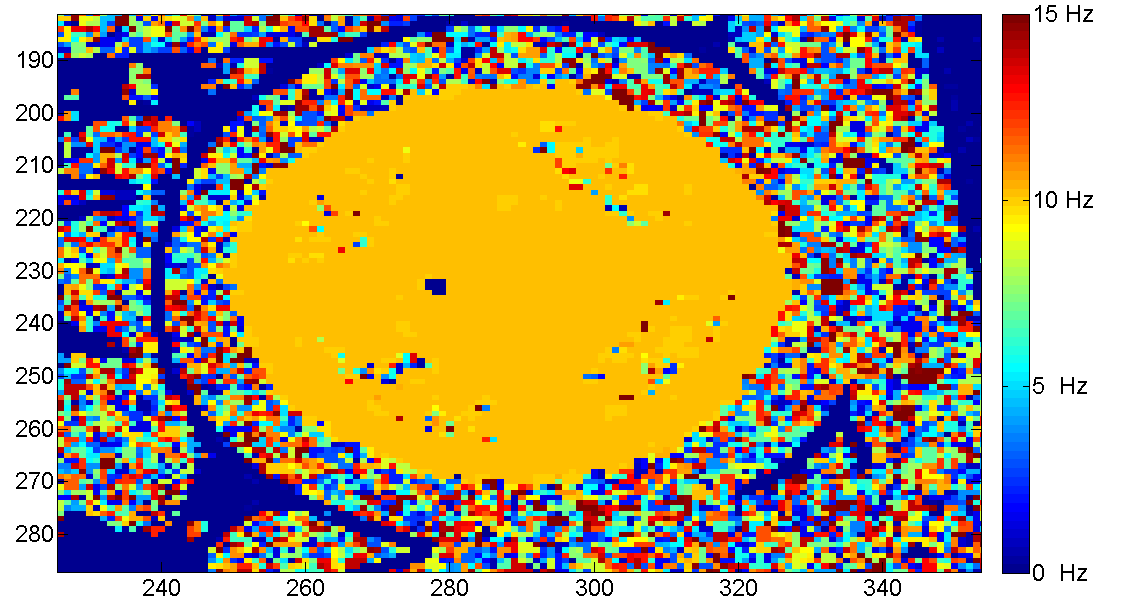
\includegraphics[width=0.5\textwidth]{Bilder/10_Hz_freq.png}}
		\end{tabular}
		\caption{Dominating frequency distribution $f_p$ of vibrations from $2~Hz$ to $10~Hz$ after $3~s$}
		\label{tbl:Dominating_freq_vs_freq}
	\end{center}
\end{table}

\newpage
\begin{table}[!h]
	\begin{center}
		\begin{tabular}{ c  p{8cm}  p{5cm}  }
			\tiny $0.6~m$
			\raisebox{-\totalheight}{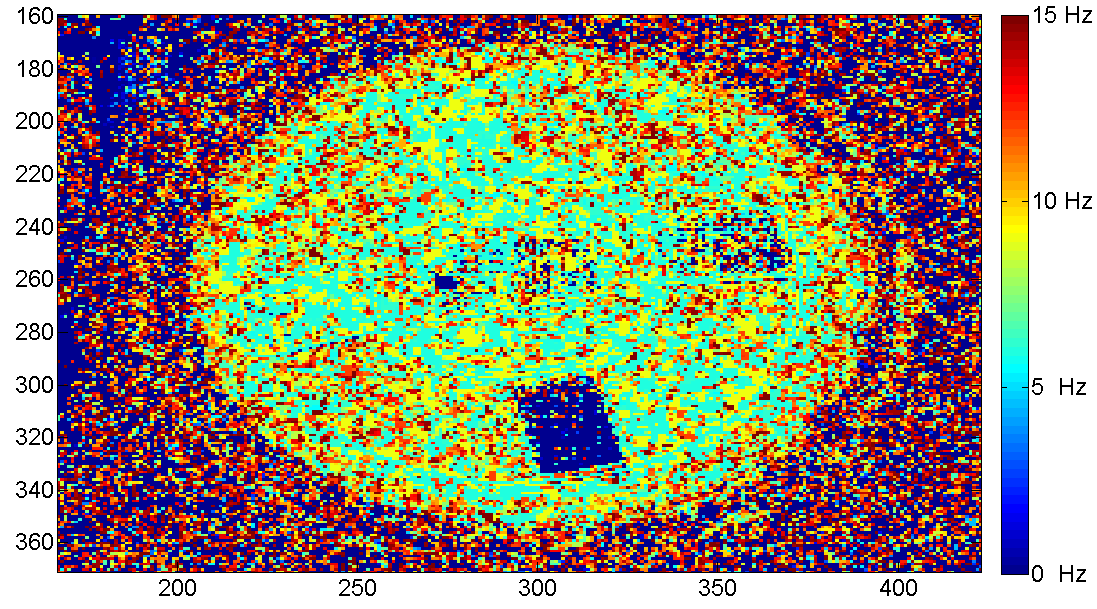
\includegraphics[width=0.5\textwidth]{Bilder/0_6m_freq_harm.png}}
			&
			\tiny $0.7~m$  
			\raisebox{-\totalheight}{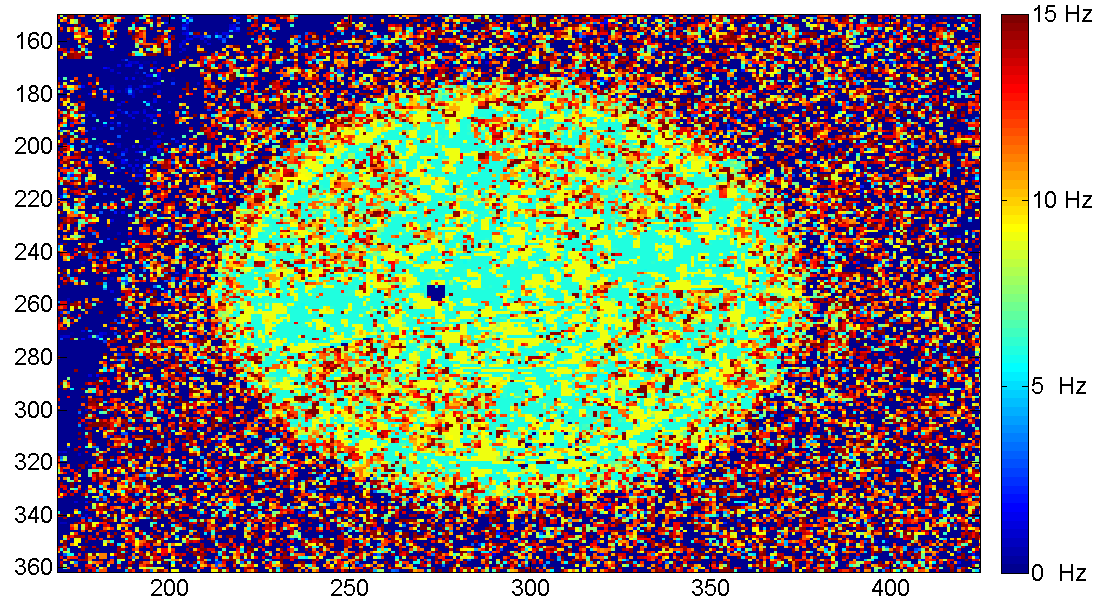
\includegraphics[width=0.5\textwidth]{Bilder/0_7m_freq_harm.png}}\\
			\tiny $0.8~m$
			\raisebox{-\totalheight}{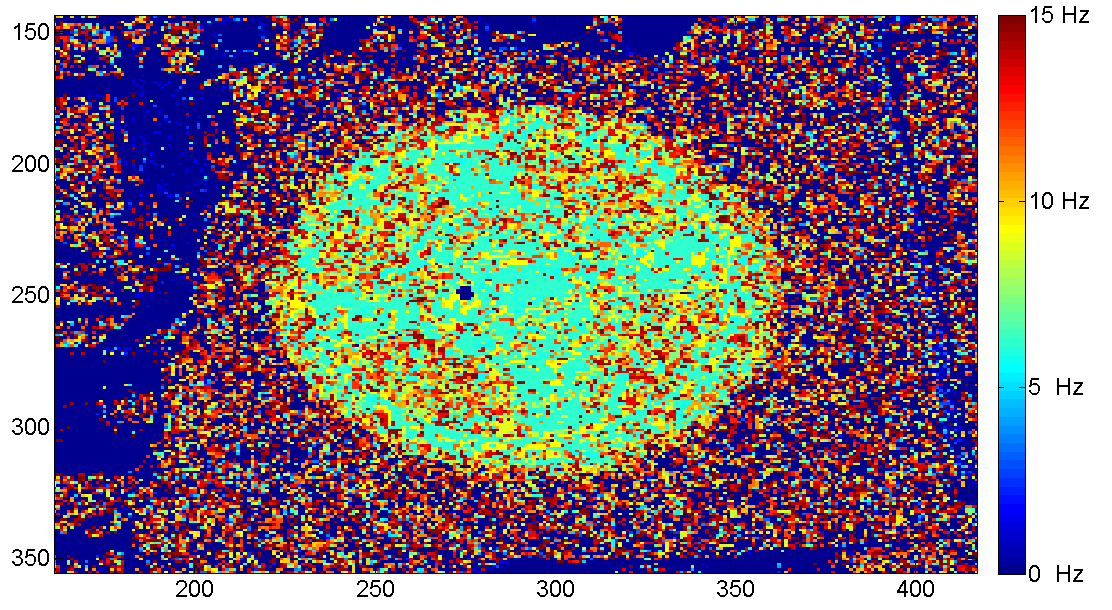
\includegraphics[width=0.5\textwidth]{Bilder/0_8m_freq_harm.png}}
			& 
			\tiny $0.9~m$
			\raisebox{-\totalheight}{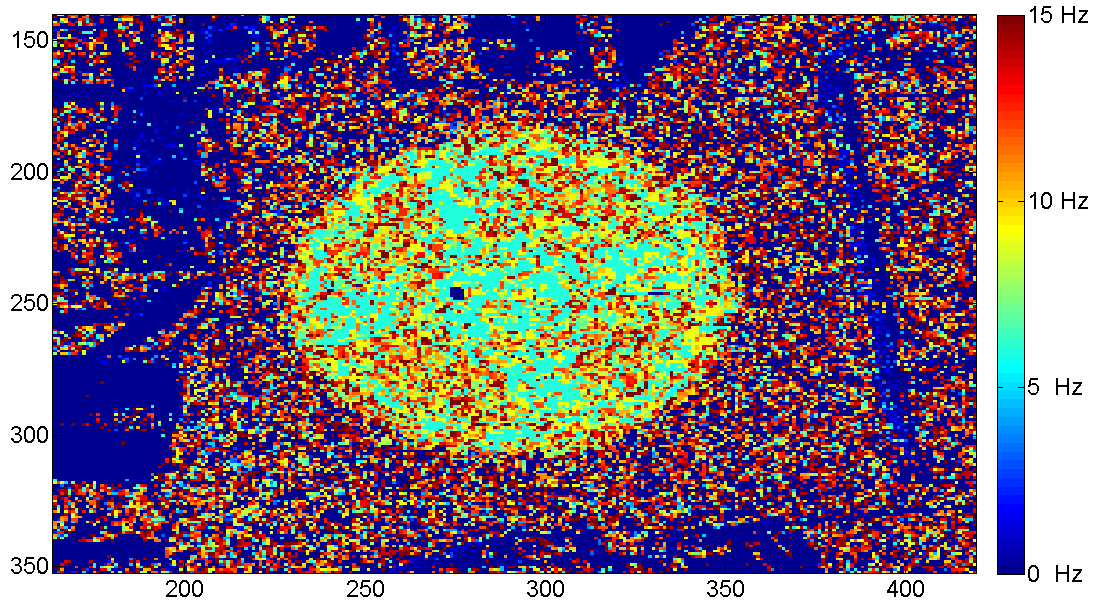
\includegraphics[width=0.5\textwidth]{Bilder/0_9m_freq_harm.png}}\\
			\tiny $1.0~m$
			\raisebox{-\totalheight}{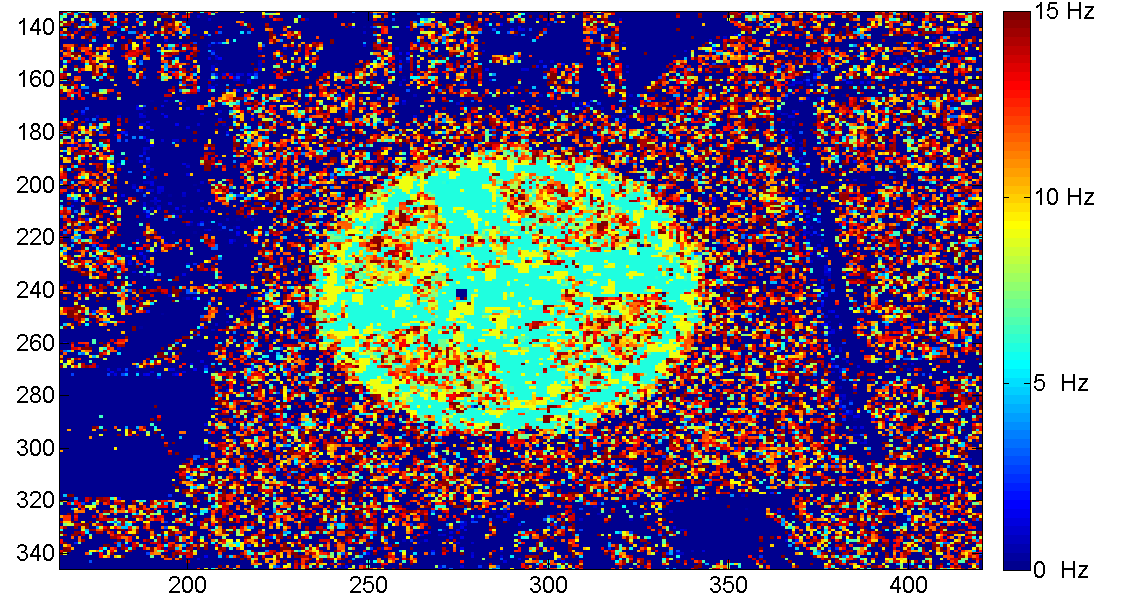
\includegraphics[width=0.5\textwidth]{Bilder/1_0m_freq_harm.png}}
			& 
			\tiny $1.1~m$
			\raisebox{-\totalheight}{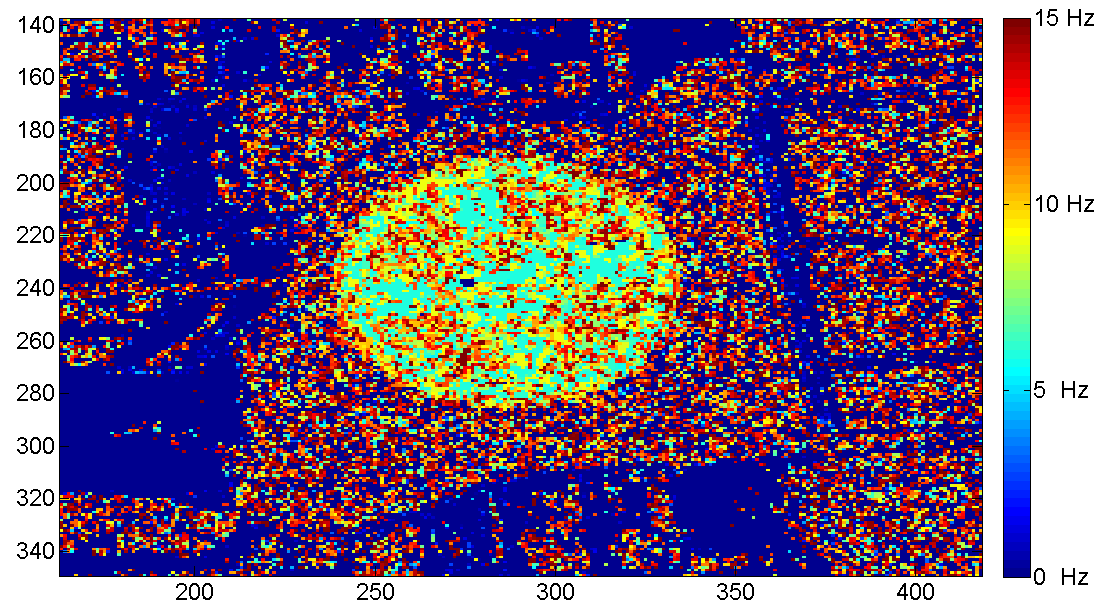
\includegraphics[width=0.5\textwidth]{Bilder/1_1m_freq_harm.png}}\\
			\tiny $1.2~m$
			\raisebox{-\totalheight}{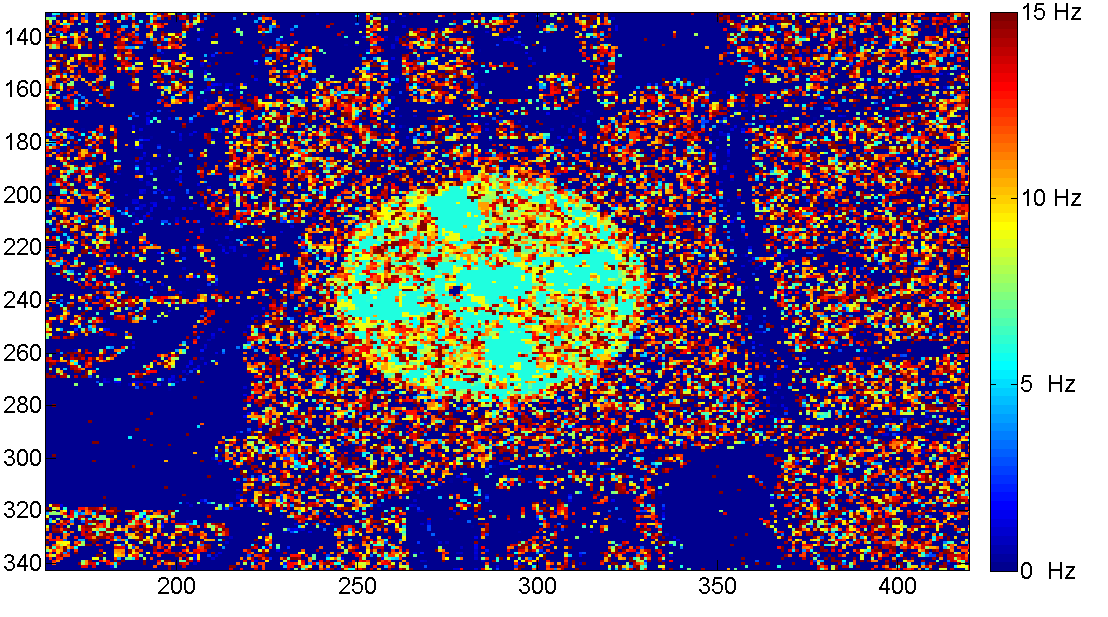
\includegraphics[width=0.5\textwidth]{Bilder/1_2m_freq_harm.png}}
			&
			\tiny $1.3~m$ 
			\raisebox{-\totalheight}{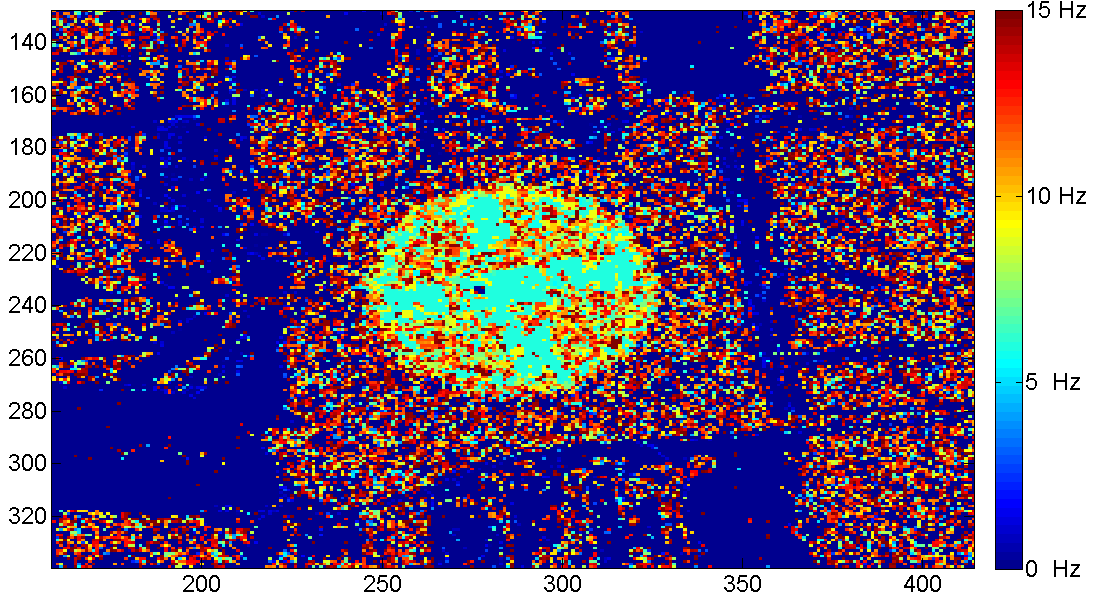
\includegraphics[width=0.5\textwidth]{Bilder/1_3m_freq_harm.png}}
		\end{tabular}
		\caption{Dominating harmonic frequency $f_{hp}$ distribution of $3~Hz$ oscillation in a distance of $0.6~m$ to $1.3~m$ after 8 s }
		\label{tbl:Dominating_harmonic_distance}
	\end{center}
\end{table}
\newpage
\begin{figure}[!h]   
	\centering
	\includegraphics[width=0.40\textwidth]{Bilder/KinectScreenshot-Color-10-58-52.png}
	\caption{Influence of $2000~W$ halogen lighting on the RGB image}
	\label{fig:KinectScreenshot-Color-10-58-52}
\end{figure}

\newpage

\begin{figure}[!h]  
	\centering
	\includegraphics[width=0.70\textwidth]{Bilder/Photodiode_measurement.jpg}
	\caption{Modulation of Kinect 2 IR lighting measured with a photodiode}
	\label{fig:Kinect2_photodiode}
\end{figure}

\begin{figure}[!h]  
	\centering
	\includegraphics[width=0.70\textwidth]{Bilder/Photodiode_measurement_kinect_3frequencies.jpg}
	\caption{Three different light intensities in one image frame}
	\label{fig:Photodiode_measurement_kinect_3frequencies}
\end{figure}

\newpage